% !TeX program = pdflatex
% !BIB program = biber
% 000_preamble.tex - Preamble for Foundations of Mathematics
% mistral/mistral-small-latest (Capability Tier 3)
\documentclass{article}

\usepackage{amsmath}
\usepackage{amssymb}
\usepackage{amsthm}

\title{Foundations of Mathematics}
\author{Autonomous Worker}
\date{\today}

\begin{document}
\maketitle
\end{document}
\renewcommand{\thechapter}{\arabic{chapter}}
\renewcommand{\chaptername}{Chapter}
\counterwithin{section}{chapter}
\addbibresource{references.bib}
\definecolor{thesislink}{rgb}{0,0.18,0.38}
\hypersetup{%
  linkcolor=thesislink,%
  citecolor=thesislink,%
  urlcolor=thesislink,%
  pdftitle={Schrodinger Semigroups and Dynamical Potentials},%
  pdfauthor={Georgy Dunaev}%
}
\title{Schr\"odinger Semigroups\\and Dynamical Potentials\\
\large Continuous kernels and quantitative parameter regularity}
\date{\today}

\begin{document}
\maketitle
\begin{abstract}
We construct the heat semigroup of the nonnegative Laplacian on
$\mathbb R^d$, prove a maximum principle and uniqueness in a Gaussian
growth class, and establish a precise measure-extension criterion for
separately continuous integral kernels. For every bounded real measurable
potential, a convergent perturbation series then produces a jointly
continuous Schr\"odinger kernel with two-sided Gaussian bounds.

For potentials generated by a Lipschitz function on a compact metric
dynamical system, we prove a quantitative Lipschitz estimate in the
dynamical parameter. Under a linear spatial growth bound for the action,
the estimate holds in every exponentially weighted supremum norm at
positive times. The proof uses a pointwise Duhamel identity and an explicit
Gaussian moment. We also treat Hölder sampling functions and construct
a family whose kernels satisfy the weighted Lipschitz estimate while
its semigroups fail to be continuous in operator norm. Translation
conventions are stated consistently:
the potential $V_z(g)=v(T(g,z))$ gives the parameter $T(g,z)$ in the
covariant kernel formula; the negative-action convention gives $T(-g,z)$.
\end{abstract}

\tableofcontents
\chapter*{Introduction and proof structure}
\addcontentsline{toc}{chapter}{Introduction and proof structure}
The object of study is the family of operators
\[
H_z=H_0+V_z,\qquad
H_0=-\sum_{j=1}^d\partial_j^2,\qquad
V_z(g)=v(T(g,z))
\]
on complex $L^2(\mathbb R^d)$. Here $Z$ is a compact metric space,
$T$ is a continuous action of $\mathbb R^d$ on $Z$, and $v$ is real
and Lipschitz. We assume
\[
d_Z(T(g,z),T(g,w))\leq C(1+|g|)d_Z(z,w).
\]
Writing $M=\|v\|_\infty$ and $L=\operatorname{Lip}(v)$, the principal
parameter estimate is
\[
\begin{split}
|k_t(z,r)-k_t(w,r)|
\leq{}&LCe^{Mt}d_Z(z,w)(4\pi t)^{-d/2}e^{-|r|^2/(4t)}\\
&\cdot\left[t\left(1+\frac{|r|}{2}\right)
                  +\frac{\pi\sqrt{2d}}8t^{3/2}\right].
\end{split}
\]
The canonical kernel is $k_t(z,r)=K_z(t,0,r)$. We prove this estimate
in Theorem~\ref{thm:dynamic_kernel_lipschitz}, after constructing the
continuous representative $K_z$ and justifying pointwise Duhamel.
Thus the estimate concerns specified continuous functions, rather than
an unspecified family of almost-everywhere kernel classes.

The development has four stages.
\begin{enumerate}
\item The Gaussian calculation and a whole-space maximum principle give
existence and uniqueness for the free heat equation in a stated growth
class.
\item The measure-extension criterion explains the functional-analytic
meaning of a separately continuous kernel. Full support is used exactly
where uniqueness requires it.
\item Bounded perturbations of the self-adjoint free Laplacian yield
Schr\"odinger semigroups. The Dyson series gives joint continuity,
Gaussian bounds, positivity, and pointwise composition. These bounds
give all $L^p$--$L^q$ smoothing estimates with $1\leq p\leq q\leq\infty$;
a separate graph-norm argument proves the Trotter product formula
strongly and uniformly on bounded time intervals.
\item Translation covariance and a Gaussian moment turn the action's
spatial Lipschitz growth into the displayed kernel estimate and its
weighted-norm consequences.
\end{enumerate}

\paragraph{Background and scope.}
The manuscript uses Lebesgue integration, dominated convergence, Fubini,
elementary multivariable calculus, Fourier--Plancherel, and the spectral
theorem for self-adjoint operators. Their precise Fourier and spectral
forms are stated where used. These standard background results are
imported; the perturbation, continuity, covariance, and parameter estimates
are proved here. General unbounded-potential perturbation theory is not
needed. In particular bounded real multiplication is handled by a direct
adjoint-domain proof of the relevant case of Kato--Rellich.

\paragraph{How the source statements fit.}
Jost's Theorem~5.1.2 is a whole-space maximum principle, from which
uniqueness follows by applying it to both signs of a difference;
Section~5.2 constructs the Gaussian solution \parencite{Jost2013PDE}.
Simon's Theorem~A.1.3 concerns separately continuous kernels, while his
Theorem~B.7.1 concerns the joint continuity relevant to Schr\"odinger
semigroups \parencite{Simon1982Semigroups}. Our measure-theoretic formulation
makes the boundedness, support, and dual-pair conventions explicit.
Kato's bounded-perturbation expansion provides another formulation of
the series method \parencite[Chapter IX, Section 2]{Kato1995Perturbation}.
The established results and the derivations in this manuscript should
not be confused with a claim of bibliographic novelty for the final
parameter estimate.

\textcite[Theorems~5.1 and~6.1]{BroderixHundertmarkLeschke2000}
treat magnetic operators with Kato-decomposable scalar potentials.
Under their local Kato convergence hypotheses and uniform small-scale
Kato control of the negative parts, potential approximation gives
convergence in $L^p\to L^q$ operator norm, $1\leq p\leq q\leq\infty$,
after multiplication by a compact-set indicator on either side,
uniformly on compact positive time intervals. When $p=q$ their time
interval may include zero. They also construct a kernel jointly
continuous in time and both interior spatial variables. Our bounded,
nonmagnetic setting supplies an explicit Lipschitz estimate for
$z\mapsto k_t(z,\cdot)$ in the norm
$\sup_r e^{a|r|}|\cdot|$, using the specified action growth bound.
These distinct continuity statements are compared without claiming
novelty for the quantitative estimate.

Both Simon and Broderix--Hundertmark--Leschke use the free operator
$-\tfrac12\sum_j\partial_j^2$. The two normalizations give
\[
\begin{array}{c|c}
\text{Free operator}&\text{Heat kernel}\\
-\tfrac12\sum_j\partial_j^2
 &(2\pi t)^{-d/2}\exp(-|r|^2/(2t))\\
-\sum_j\partial_j^2
 &(4\pi t)^{-d/2}\exp(-|r|^2/(4t)).
\end{array}
\]
We use the second convention throughout; constants must be compared
with this normalization in mind.

\chapter{The free heat equation}
\def\topic{The free heat equation and uniqueness}
\ifdefined\MyHeaderIncluded
\else
\def\qwertyflag{true}

\ifdefined\MyHeaderIncluded

\else
  \newcommand{\foobar}{FooBar}
  \def\MyHeaderIncluded{true}
% if is till the end of the file

\documentclass[10pt,a4paper]{article}
\usepackage[utf8]{inputenc}
%\usepackage[german]{babel}
%\usepackage[cyrillic]{babel}
\usepackage[T1]{fontenc}
%\usepackage[T2A]{fontenc}
%\usepackage[english, russian]{babel}
\usepackage{amsmath}
\usepackage{amsfonts}
\usepackage{amssymb}
\usepackage{amsthm}
\usepackage{mathtools} %coloneqq

\usepackage{bussproofs} %

%\renewcommand{\thesubsection}{\arabic{subsection}}
%\newtheorem{thm}{Theorem}[section]
%\renewcommand{\thethm}{\arabic{subsection}.\arabic{thm}}

\usepackage{thmtools}
\usepackage{hyperref}
\hypersetup{
    colorlinks=true,
    linkcolor=blue,
    filecolor=magenta,      
    urlcolor=cyan,
    pdftitle={Overleaf Example},
    %pdfpagemode=FullScreen,
    }
%\usepackage{stix-type1}%\turnediota
\theoremstyle{definition}

\newtheorem{constructor}{Constructor}[section]
\newtheorem{iaxiom}{Axiom}
\newtheorem{axiom}{Axiom}
\newtheorem*{axiom*}{Axiom}
\newtheorem{definition}{Definition}[section]
\newtheorem*{definition*}{Definition}
\newtheorem{remark}{Remark}[section]
\newtheorem*{remark*}{Remark}
\newtheorem{recall}{Recall}[section]
\newtheorem*{recall*}{Recall}

\newtheorem{lemma}{Lemma}[section]
\newtheorem{theorem}{Theorem}[section]
\newtheorem*{theorem*}{Theorem}
\newtheorem{note}{Note}[section]
\usepackage{etoolbox}

%\newcommand*{\@Dashv}[2]{%
%  \reflectbox{$\m@th#1#2$}%
%}
\newcommand*{\separation}[3]{% 1)binder, 2)set, 3)condition
  \{#1\in #2: #3\}
}

% https://www.freecodecamp.org/news/simple-regex-tricks-for-beginners-3acb3fa257cb/
%  \\mathcal\{T\} |---> \topology
%  \\mathcal\{([^\}]*)\}   |--->  $1
\newcommand{\AND}{\ \ \&\ \ }
\newcommand{\any}{\mathrm{\ any}}
\newcommand{\borel}{\mathcal{B}}
\newcommand{\can}{\mathrm{can}}
\newcommand{\canonize}{\mathrm{canonize}}
\newcommand{\closure}{\mbox{cl}}
\newcommand{\complex}{\mathbb{C}}
\newcommand{\converges}{\longrightarrow}
\newcommand{\countable}{\mbox{\ countable}}
\newcommand{\ldefined}{\mbox{\ defined}}
\newcommand{\dom}{\mbox{dom}}
\newcommand{\Dom}{\mbox{Dom}}
\newcommand{\Done}{\noindent \textbf{Done.}\\}
\newcommand{\lexists}{\mbox{\ exists}}
\newcommand{\lforall}{\mbox{\ forall}}
\newcommand{\lunique}{\mbox{\ unique}}
\newcommand{\family}{\mathrm{\ family}}
\newcommand{\Fm}{\mathrm{Fm}}
\newcommand{\FuncSymb}{\mathrm{FuncSymb}}
\newcommand{\function}{\mathrm{\ function}}
\newcommand{\functional}{\mbox{\ functional}}
\newcommand{\IFF}{\ \Longleftrightarrow\ }
\renewcommand{\iff}{\ \longleftrightarrow\ }
\newcommand{\IMPLIES}{\ \Longrightarrow\ }
\renewcommand{\implies}{\ \longrightarrow\ }
\newcommand{\Inf}{\mathrm{Inf}}
\newcommand{\injective}{\mbox{\ injective}}
\newcommand{\injection}{\mbox{\ injection}}
\newcommand{\interior}{\mbox{int}}
\newcommand{\intersection}{\bigcap}
\newcommand{\isempty}{\mathrm{\ empty}}
\newcommand{\LB}{\mathrm{LB}}
\newcommand{\nghbset}{\mathcal{N}}
\newcommand{\nonempty}{\mathrm{\ nonempty}}
\newcommand{\Ord}{\mathrm{Ord}}
\newcommand{\power}{\mathcal{P}}
\newcommand{\pr}{\mathrm{pr}}
\newcommand{\fst}{\mathrm{fst}}
\newcommand{\snd}{\mathrm{snd}}
\newcommand{\PredSymb}{\mathrm{PredSymb}}
\newcommand{\Proof}{\noindent \textbf{Proof.}\\}
\newcommand{\ran}{\mathrm{ran}}
\newcommand{\Ran}{\mathrm{Ran}}
\newcommand{\real}{\mathbb{R}}
\newcommand{\relation}{\mathrm{\ relation}}
\newcommand{\set}{\mathrm{\ set}}
\newcommand{\singleton}{\mathrm{\ singleton}}
\newcommand{\semantics}{\mathrm{semantics}}
\newcommand{\semialgebra}{\mathcal{S}}
\newcommand{\Sup}{\mathrm{Sup}}
\newcommand{\surjective}{\mbox{\ surjective\ on\ }}
\newcommand{\Term}{\mathrm{Term}}
\newcommand{\Type}{\mathrm{Type}}
\newcommand{\topology}{\mathcal{T}}
\newcommand{\total}{\mbox{\ total\ on\ }}
\newcommand{\transitive}{\mathrm{\ transitive}}
\newcommand{\union}{\bigcup}
\newcommand{\lTrue}{\mathrm{True}}
\newcommand{\lFalse}{\mathrm{False}}
\newcommand{\lUncertain}{\mathrm{Uncertain}}
\newcommand{\lif}{\mathrm{if}}
\newcommand{\lthen}{\mathrm{then}}
\newcommand{\lelse}{\mathrm{else}}
\newcommand{\lexception}{\mathrm{exception}}
\newcommand{\lundef}{\mathrm{undef}}
\newcommand{\univocal}{\mathrm{\ univocal}}
\newcommand{\univocalat}{\mathrm{\ univocal\ at\ }}
\newcommand{\UB}{\mathrm{UB}}
\newcommand{\Un}{\mathcal{U}}
\newcommand{\Var}{\mathrm{Var}}

\newcommand{\notvarphi}{\phi}
\renewcommand{\phi}{\varphi}

\newcommand{\comment}[1]{\quad\mbox{(#1)}}
% local commands
%\preto\section{\undef\blipo} %etoolbox
\preto\subsection{\undef\blipo} %etoolbox
% https://tex.stackexchange.com/questions/105684/limit-macro-newcommand-scope-to-section
\usepackage{graphicx}
\usepackage{authblk}

\setlength\parindent{0pt} % whole doc of \noindent
\usepackage{soul}
%\usepackage{mathgl}

\fi % guard
\ifdefined\topic
\else
\def\topic{No Titel}
\fi
\title{\topic}
\author[1]{Georgy Dunaev}
\begin{document}
\maketitle
\fi
\section{The free heat equation and uniqueness}
\label{sec:free_heat_equation}
Work on $\mathbb R^d$, $d\geq1$, with Lebesgue measure. In this
chapter write $L=\sum_{j=1}^d\partial_j^2$ for the differential
Laplacian. Thus the nonnegative operator used in the next chapters is
$H_0=-L$, and its heat equation is $u_t=Lu$.
We use elementary multivariable differentiation, the Gaussian integral,
and dominated convergence. The point of the uniqueness argument is its
explicit growth class: a whole-space initial-value problem does not
acquire unrestricted uniqueness from a bounded-domain maximum principle.
Jost's Theorem~5.1.2 is precisely a maximum principle with such a
growth restriction, while his Section~5.2 constructs the fundamental
solution \parencite{Jost2013PDE}.

\subsection{The Gaussian and its convolution law}
For $t>0$ put
\[
p_t(x)=(4\pi t)^{-d/2}\exp\bigl(-|x|^2/(4t)\bigr).
\]
\begin{lemma}[Elementary Gaussian identities]
\label{lem:free_gaussian_convolution}
The function $p_t$ is positive, has integral one, satisfies
$\partial_tp_t=Lp_t$, and obeys
\[
\int_{\mathbb R^d}p_s(x-z)p_t(z-y)\,dz=p_{s+t}(x-y)
\qquad(s,t>0).
\]
\end{lemma}
\Proof
The substitution $x=2\sqrt t\,q$ and the product formula for the
one-dimensional Gaussian integral give $\int p_t=1$. Direct
coordinate differentiation gives
\[
\partial_tp_t(x)=\left(-\frac d{2t}+\frac{|x|^2}{4t^2}\right)p_t(x),
\qquad
\partial_j^2p_t(x)=\left(-\frac1{2t}+\frac{x_j^2}{4t^2}\right)p_t(x),
\]
so summing the second identity proves the differential equation.
For convolution complete the square:
\[
\frac{|x-z|^2}{s}+\frac{|z-y|^2}{t}
=\frac{s+t}{st}\left|z-\frac{tx+sy}{s+t}\right|^2
 +\frac{|x-y|^2}{s+t}.
\]
The remaining Gaussian integral is
$(4\pi st/(s+t))^{d/2}$. Multiplying by the two normalization
factors yields the asserted formula. All these integrals are absolutely
convergent; their positive integrands also permit Tonelli's theorem.
\Done

\begin{lemma}[The Gaussian Fourier multiplier]
\label{lem:gaussian_fourier_multiplier}
For the unitary Fourier normalization
$\widehat f(\xi)=(2\pi)^{-d/2}\int e^{-ix\cdot\xi}f(x)\,dx$,
\[
\widehat{p_t}(\xi)=(2\pi)^{-d/2}e^{-t|\xi|^2}.
\]
Consequently convolution by $p_t$ has Fourier multiplier
$e^{-t|\xi|^2}$.
\end{lemma}
\Proof
In one dimension let
$F(a)=\int_{\mathbb R}e^{-x^2/(4t)}e^{-iax}\,dx$.
The integrable function $|x|e^{-x^2/(4t)}$ permits differentiation
under the integral. Since
$x e^{-x^2/(4t)}=-2t\,\frac{d}{dx}e^{-x^2/(4t)}$,
integration by parts, with vanishing Gaussian boundary terms, gives
\[
F'(a)=2it\int_{\mathbb R}
 \frac{d}{dx}\bigl(e^{-x^2/(4t)}\bigr)e^{-iax}\,dx
 =-2taF(a).
\]
Together with $F(0)=\sqrt{4\pi t}$, this scalar differential
equation gives $F(a)=\sqrt{4\pi t}\,e^{-ta^2}$.
Taking the product in $d$ coordinates proves the displayed transform.
For an integrable function $f$, Fubini applied to the convolution
integral gives
$\widehat{p_t*f}=(2\pi)^{d/2}\widehat{p_t}\,\widehat f$,
which proves the multiplier assertion on integrable functions.
For $f\in L^2$, Jensen's inequality for the probability density
$p_t$ and Tonelli give
\[
\|p_t*f\|_2^2
\leq\int_{\mathbb R^d}\int_{\mathbb R^d}
          p_t(z)|f(x-z)|^2\,dz\,dx=\|f\|_2^2.
\]
Approximation by $L^1\cap L^2$ functions and Fourier--Plancherel
therefore extend the multiplier identity to $L^2$.
\Done

\begin{theorem}[The solution for bounded continuous initial data]
\label{thm:free_heat_bounded_data}
If $f:\mathbb R^d\to\mathbb R$ is bounded and continuous, then
\[
u(x,t)=\int_{\mathbb R^d}p_t(x-y)f(y)\,dy\quad(t>0),
\qquad u(x,0)=f(x)
\]
is continuous on $\mathbb R^d\times[0,\infty)$, smooth for $t>0$,
and solves $u_t=Lu$. Moreover
$|u(x,t)|\leq\|f\|_\infty$ and $u(\cdot,t)\to f$ locally
uniformly as $t\downarrow0$. The operators $P_tf=u(\cdot,t)$ satisfy
$P_sP_t=P_{s+t}$.
\end{theorem}
\Proof
Absolute convergence and the bound follow from $\int p_t=1$.
Every spatial or time derivative of the Gaussian is a polynomial
in $x-y$ times a Gaussian, with coefficients bounded when $t$ stays
in a compact subinterval of $(0,\infty)$. For $x$ in a fixed compact
set these derivatives admit an integrable majorant in $y$ of the form
$C(1+|y|^N)e^{-c|y|^2}$. Differentiation under the integral is therefore
legitimate to every order;
Lemma~\ref{lem:free_gaussian_convolution} gives the equation.

For a compact set $K$ and a number $\varepsilon>0$, continuity of
$f$ on a compact neighbourhood of $K$ supplies $\delta>0$ such that
$|f(x-z)-f(x)|<\varepsilon$ whenever $x\in K$ and $|z|<\delta$.
Consequently
\[
\sup_{x\in K}|P_tf(x)-f(x)|
\leq\varepsilon+2\|f\|_\infty
                 \int_{|z|\geq\delta}p_t(z)\,dz.
\]
After $z=\sqrt t\,q$, the last integral is a Gaussian tail outside
$|q|\geq\delta/\sqrt t$, and tends to zero. This proves the initial
trace and continuity at $t=0$. Fubini, boundedness of $f$, and the
Gaussian convolution identity prove the semigroup law. For complex
initial data apply the construction to real and imaginary parts.
\Done

\subsection{Why the growth condition gives uniqueness}
A classical subsolution on a time slab $[0,T]$ means a real function
continuous up to $t=0$, with continuous second spatial derivatives
and first time derivative for $t>0$, satisfying $u_t-Lu\leq0$.
At the final time derivatives can be understood from the left.

\begin{lemma}[Maximum principle on a bounded cylinder]
\label{lem:heat_cylinder_maximum}
Let $B_R=\{x:|x|<R\}$ and let $u$ be a classical subsolution on
$\overline B_R\times[0,T]$. Its supremum is at most its supremum
on the parabolic boundary
$(\overline B_R\times\{0\})\cup(\partial B_R\times[0,T])$.
\end{lemma}
\Proof
For $\eta>0$ consider $w=u-\eta t$, which satisfies
$w_t-Lw\leq-\eta$. If $w$ exceeded the parabolic-boundary supremum
of $u$, compactness would give a maximum at $(x_0,t_0)$ with
$x_0\in B_R$ and $t_0>0$. At this point $Lw\leq0$ and
$w_t\geq0$: at $t_0=T$ the latter follows from the left derivative,
and at an interior time it is zero. This contradicts the strict
differential inequality. Thus $u\leq\sup_{\partial_p}u+\eta T$;
letting $\eta\downarrow0$ proves the claim.
\Done

\begin{theorem}[Whole-space maximum principle with Gaussian growth]
\label{thm:heat_gaussian_growth_maximum}
Let $T>0$ be finite and let $u$ be a classical subsolution on
$\mathbb R^d\times[0,T]$. Suppose there are $M,\lambda>0$ with
\[
u(x,t)\leq M e^{\lambda|x|^2}\quad(0\leq t\leq T),
\qquad m=\sup_{x\in\mathbb R^d}u(x,0)<\infty.
\]
Then $u(x,t)\leq m$ throughout the slab.
\end{theorem}
\Proof
First suppose the slab length $S$ satisfies $S<1/(4\lambda)$.
Choose $\tau$ with $S<\tau<1/(4\lambda)$ and define
\[
b(x,t)=(\tau-t)^{-d/2}
       \exp\left(\frac{|x|^2}{4(\tau-t)}\right),\qquad0\leq t\leq S.
\]
Direct differentiation gives $b_t=Lb$. For a fixed $\varepsilon>0$,
$w=u-m-\varepsilon b$ is a subsolution and $w(x,0)\leq0$.
On $|x|=R$ the uniform bound
\[
w(x,t)\leq M e^{\lambda R^2}+|m|
 -\varepsilon\tau^{-d/2}e^{R^2/(4\tau)}
\]
is negative for all sufficiently large $R$, since
$1/(4\tau)>\lambda$. The bounded-cylinder lemma implies $w\leq0$
inside every such cylinder. For each fixed $(x,t)$ choose a cylinder
containing it and then let $\varepsilon\downarrow0$. Hence $u\leq m$
on this short slab.

For an arbitrary finite $T$, partition $[0,T]$ into finitely many
slabs of length less than $1/(4\lambda)$. The same growth constants
work on each translated slab. The first step bounds the initial
values of the next slab by $m$, so induction gives the conclusion
on all of them. No limit as a spatial boundary tends to infinity
has been taken without the barrier estimate.
\Done

\begin{corollary}[Uniqueness in the stated growth class]
\label{cor:heat_gaussian_growth_uniqueness}
Two real classical solutions with the same continuous initial data
coincide if, on every finite time slab, each satisfies an absolute
bound $|u(x,t)|\leq M e^{\lambda|x|^2}$ for some slab-dependent
constants. In particular the bounded solution in
Theorem~\ref{thm:free_heat_bounded_data} is unique among bounded
classical solutions. The same conclusion holds for complex solutions.
\end{corollary}
\Proof
On a fixed slab the difference $w$ has zero initial data and an
absolute Gaussian-growth bound, after increasing the two constants
if necessary. Apply the maximum principle to $w$ and to $-w$.
Both are at most zero, hence $w=0$. For complex solutions apply this
to the real and imaginary parts of the difference.
\Done

The Gaussian here is a kernel of the heat semigroup, not a statement
that the differential operator $L$ has only one distributional kernel
or that all unrestricted classical Cauchy problems are unique.
The $L^2$ interpretation uses Fourier--Plancherel and the spectral
calculus in Section~\ref{sec:bounded_schrodinger}; its initial condition
is an $L^2$ limit, whereas the present theorem assumes continuous
initial data and proves a locally uniform limit.
\ifdefined\qwertyflag
\undef\qwertyflag
\end{document}
\fi

\chapter{An abstract kernel criterion}
\def\topic{Continuous integral kernels}
\ifdefined\MyHeaderIncluded
\else
\def\qwertyflag{true}

\ifdefined\MyHeaderIncluded

\else
  \newcommand{\foobar}{FooBar}
  \def\MyHeaderIncluded{true}
% if is till the end of the file

\documentclass[10pt,a4paper]{article}
\usepackage[utf8]{inputenc}
%\usepackage[german]{babel}
%\usepackage[cyrillic]{babel}
\usepackage[T1]{fontenc}
%\usepackage[T2A]{fontenc}
%\usepackage[english, russian]{babel}
\usepackage{amsmath}
\usepackage{amsfonts}
\usepackage{amssymb}
\usepackage{amsthm}
\usepackage{mathtools} %coloneqq

\usepackage{bussproofs} %

%\renewcommand{\thesubsection}{\arabic{subsection}}
%\newtheorem{thm}{Theorem}[section]
%\renewcommand{\thethm}{\arabic{subsection}.\arabic{thm}}

\usepackage{thmtools}
\usepackage{hyperref}
\hypersetup{
    colorlinks=true,
    linkcolor=blue,
    filecolor=magenta,      
    urlcolor=cyan,
    pdftitle={Overleaf Example},
    %pdfpagemode=FullScreen,
    }
%\usepackage{stix-type1}%\turnediota
\theoremstyle{definition}

\newtheorem{constructor}{Constructor}[section]
\newtheorem{iaxiom}{Axiom}
\newtheorem{axiom}{Axiom}
\newtheorem*{axiom*}{Axiom}
\newtheorem{definition}{Definition}[section]
\newtheorem*{definition*}{Definition}
\newtheorem{remark}{Remark}[section]
\newtheorem*{remark*}{Remark}
\newtheorem{recall}{Recall}[section]
\newtheorem*{recall*}{Recall}

\newtheorem{lemma}{Lemma}[section]
\newtheorem{theorem}{Theorem}[section]
\newtheorem*{theorem*}{Theorem}
\newtheorem{note}{Note}[section]
\usepackage{etoolbox}

%\newcommand*{\@Dashv}[2]{%
%  \reflectbox{$\m@th#1#2$}%
%}
\newcommand*{\separation}[3]{% 1)binder, 2)set, 3)condition
  \{#1\in #2: #3\}
}

% https://www.freecodecamp.org/news/simple-regex-tricks-for-beginners-3acb3fa257cb/
%  \\mathcal\{T\} |---> \topology
%  \\mathcal\{([^\}]*)\}   |--->  $1
\newcommand{\AND}{\ \ \&\ \ }
\newcommand{\any}{\mathrm{\ any}}
\newcommand{\borel}{\mathcal{B}}
\newcommand{\can}{\mathrm{can}}
\newcommand{\canonize}{\mathrm{canonize}}
\newcommand{\closure}{\mbox{cl}}
\newcommand{\complex}{\mathbb{C}}
\newcommand{\converges}{\longrightarrow}
\newcommand{\countable}{\mbox{\ countable}}
\newcommand{\ldefined}{\mbox{\ defined}}
\newcommand{\dom}{\mbox{dom}}
\newcommand{\Dom}{\mbox{Dom}}
\newcommand{\Done}{\noindent \textbf{Done.}\\}
\newcommand{\lexists}{\mbox{\ exists}}
\newcommand{\lforall}{\mbox{\ forall}}
\newcommand{\lunique}{\mbox{\ unique}}
\newcommand{\family}{\mathrm{\ family}}
\newcommand{\Fm}{\mathrm{Fm}}
\newcommand{\FuncSymb}{\mathrm{FuncSymb}}
\newcommand{\function}{\mathrm{\ function}}
\newcommand{\functional}{\mbox{\ functional}}
\newcommand{\IFF}{\ \Longleftrightarrow\ }
\renewcommand{\iff}{\ \longleftrightarrow\ }
\newcommand{\IMPLIES}{\ \Longrightarrow\ }
\renewcommand{\implies}{\ \longrightarrow\ }
\newcommand{\Inf}{\mathrm{Inf}}
\newcommand{\injective}{\mbox{\ injective}}
\newcommand{\injection}{\mbox{\ injection}}
\newcommand{\interior}{\mbox{int}}
\newcommand{\intersection}{\bigcap}
\newcommand{\isempty}{\mathrm{\ empty}}
\newcommand{\LB}{\mathrm{LB}}
\newcommand{\nghbset}{\mathcal{N}}
\newcommand{\nonempty}{\mathrm{\ nonempty}}
\newcommand{\Ord}{\mathrm{Ord}}
\newcommand{\power}{\mathcal{P}}
\newcommand{\pr}{\mathrm{pr}}
\newcommand{\fst}{\mathrm{fst}}
\newcommand{\snd}{\mathrm{snd}}
\newcommand{\PredSymb}{\mathrm{PredSymb}}
\newcommand{\Proof}{\noindent \textbf{Proof.}\\}
\newcommand{\ran}{\mathrm{ran}}
\newcommand{\Ran}{\mathrm{Ran}}
\newcommand{\real}{\mathbb{R}}
\newcommand{\relation}{\mathrm{\ relation}}
\newcommand{\set}{\mathrm{\ set}}
\newcommand{\singleton}{\mathrm{\ singleton}}
\newcommand{\semantics}{\mathrm{semantics}}
\newcommand{\semialgebra}{\mathcal{S}}
\newcommand{\Sup}{\mathrm{Sup}}
\newcommand{\surjective}{\mbox{\ surjective\ on\ }}
\newcommand{\Term}{\mathrm{Term}}
\newcommand{\Type}{\mathrm{Type}}
\newcommand{\topology}{\mathcal{T}}
\newcommand{\total}{\mbox{\ total\ on\ }}
\newcommand{\transitive}{\mathrm{\ transitive}}
\newcommand{\union}{\bigcup}
\newcommand{\lTrue}{\mathrm{True}}
\newcommand{\lFalse}{\mathrm{False}}
\newcommand{\lUncertain}{\mathrm{Uncertain}}
\newcommand{\lif}{\mathrm{if}}
\newcommand{\lthen}{\mathrm{then}}
\newcommand{\lelse}{\mathrm{else}}
\newcommand{\lexception}{\mathrm{exception}}
\newcommand{\lundef}{\mathrm{undef}}
\newcommand{\univocal}{\mathrm{\ univocal}}
\newcommand{\univocalat}{\mathrm{\ univocal\ at\ }}
\newcommand{\UB}{\mathrm{UB}}
\newcommand{\Un}{\mathcal{U}}
\newcommand{\Var}{\mathrm{Var}}

\newcommand{\notvarphi}{\phi}
\renewcommand{\phi}{\varphi}

\newcommand{\comment}[1]{\quad\mbox{(#1)}}
% local commands
%\preto\section{\undef\blipo} %etoolbox
\preto\subsection{\undef\blipo} %etoolbox
% https://tex.stackexchange.com/questions/105684/limit-macro-newcommand-scope-to-section
\usepackage{graphicx}
\usepackage{authblk}

\setlength\parindent{0pt} % whole doc of \noindent
\usepackage{soul}
%\usepackage{mathgl}

\fi % guard
\ifdefined\topic
\else
\def\topic{No Titel}
\fi
\title{\topic}
\author[1]{Georgy Dunaev}
\begin{document}
\maketitle
\fi
\section{A criterion for separately continuous kernels}
\label{sec:continuous_kernel_criterion}
The criterion below proves a locally finite Radon-measure version of
Simon's Theorem~A.1.3 \parencite{Simon1982Semigroups}, with boundedness of
the kernel explicit. The source uses Baire measures, asks for a
norm-continuous and weakly continuous extension, and imposes full
support for uniqueness. We retain the existence criterion without
full support, and state precisely where support is needed. Its
conclusion is separate continuity, not joint continuity. We give the
proof, including the dual-pair argument needed on a noncompact space.

\subsection{Measures, representatives, and the dual pair}
Let $(X,d)$ be a nonempty separable locally compact metric space, and let
$\nu$ be a positive locally finite Radon measure on $X$. Write
$C_b(X)$ for the complex bounded continuous functions, with supremum
norm, and $\mathcal M(X)$ for the finite complex Radon measures, with
total variation norm. A function $f\in L^1(X,\nu)$ determines the
measure $f\nu\in\mathcal M(X)$, with
$\|f\nu\|_{\mathrm{TV}}=\|f\|_1$. Local compactness and separability
make $X$ a countable union of compact sets; in particular $\nu$ is
$\sigma$-finite. The next lemma justifies the Radon property of the
finite density measures, including for the wider measure convention
discussed below. All measures here are on the Borel sets. In this
metric setting the Baire and Borel sigma algebras coincide: each closed
set is the zero set of its continuous distance function.

\begin{lemma}[Regularity of the finite measures used here]
\label{lem:kernel_finite_measure_regularity}
Every finite positive Borel measure $\mu$ on $X$ is outer regular
by open sets and inner regular by compact sets. Consequently every
finite complex Borel measure on $X$ is a finite Radon measure.
\end{lemma}
\begin{proof}
Separability and metrizability give a countable base. Local compactness
then gives a countable cover by relatively compact open sets: choose
a relatively compact neighborhood at each point and extract a
countable subcover using the base. Finite unions of their closures
form increasing compact sets $K_n$ with union $X$.

We first establish approximation by closed and open sets. Let
$\mathcal R$ be the class of Borel sets $E$ for which, for every
$\epsilon>0$, there are a closed $F$ and an open $G$ with
$F\subseteq E\subseteq G$ and $\mu(G\setminus F)<\epsilon$.
Every open set $G\ne X$ belongs to $\mathcal R$: the closed sets
$\{x:d(x,X\setminus G)\geq1/n\}$ increase to $G$, and continuity
from below gives the required approximation. The set $X$ itself is
immediate. The class $\mathcal R$ is closed under complements by
interchanging the complements of $F,G$.

For $E=\bigcup_{j\geq1}E_j$ with $E_j\in\mathcal R$, choose
$F_j\subseteq E_j\subseteq G_j$ with
$\mu(G_j\setminus F_j)<\epsilon 2^{-j}/3$. Since $\mu$ is finite,
choose $N$ with
$\mu(E\setminus\bigcup_{j\leq N}E_j)<\epsilon/3$.
Then $F=\bigcup_{j\leq N}F_j$ is closed,
$G=\bigcup_{j\geq1}G_j$ is open, and
\[
\begin{aligned}
\mu(G\setminus F)
&\leq\sum_{j\geq1}\mu(G_j\setminus E_j)
 +\mu\left(E\setminus\bigcup_{j\leq N}E_j\right)\\
&\quad +\sum_{j\leq N}\mu(E_j\setminus F_j)<\epsilon.
\end{aligned}
\]
Thus $\mathcal R$ is a sigma algebra containing the open sets, so it
contains every Borel set. For a closed inner approximant $F$,
$F\cap K_n$ is compact and increases to $F$; continuity from below
therefore improves closed inner approximation to compact inner
approximation. The same argument applied to the finite positive
total variation of a complex measure proves the final assertion.
\end{proof}

Use the bilinear pairing
\[
\langle\mu,g\rangle=\int_X g\,d\mu,
\qquad \mu\in\mathcal M(X),\quad g\in C_b(X).
\]
For $x\in X$, the Dirac measure $\delta_x$ is the unit point mass at
$x$, so $\langle\delta_x,g\rangle=g(x)$.
Here $\sigma(\mathcal M,C_b)$ means convergence against every fixed
$g\in C_b$, and $\sigma(C_b,\mathcal M)$ means convergence against
every fixed $\mu\in\mathcal M$. These definitions apply to nets,
not only to sequences. They specify a dual pair; they do not identify
$\mathcal M(X)$ with the full Banach dual of $C_b(X)$, an identification
that is generally false on a noncompact space.
For completeness, the pairing separates both spaces. Dirac measures
separate continuous functions. If a finite complex measure integrates
every bounded continuous function to zero, apply this to
$\max(0,1-n d(x,F))$ for each nonempty closed $F$. Dominated convergence
gives $\mu(F)=0$. Closed inner approximation with respect to $|\mu|$
then gives $\mu(E)=0$ for every Borel $E$, so $\mu=0$.

Let $J:C_b(X)\to L^\infty(X,\nu)$ take the almost-everywhere class.
A bounded operator $T:L^1(\nu)\to L^\infty(\nu)$ has an extension
$S:\mathcal M(X)\to C_b(X)$ in the sense used here if
\[
J(S(f\nu))=Tf\qquad(f\in L^1(\nu)).
\]
This is an equality of equivalence classes. Full support means that
every nonempty open subset of $X$ has positive $\nu$-measure.
If $\nu$ has full support,
$J$ is injective and isometric: a continuous function exceeding a bound
at one point exceeds it on an open set of positive measure. Without
full support, continuous representatives need not be unique.

\begin{lemma}[Continuous linear functionals for the specified weak topology]
\label{lem:kernel_weak_dual}
Every continuous complex-linear functional $F$ on
$(\mathcal M(X),\sigma(\mathcal M,C_b))$ has the form
$F(\mu)=\int g\,d\mu$ for a unique $g\in C_b(X)$.
\end{lemma}
\begin{proof}
Continuity at zero gives $g_1,\ldots,g_n\in C_b(X)$ and
$\epsilon>0$ such that $|\int g_j\,d\mu|<\epsilon$ for all $j$
implies $|F(\mu)|<1$. If all those integrals vanish, every scalar
multiple of $\mu$ belongs to this neighborhood; linearity forces
$F(\mu)=0$. Thus $F$ factors through the map
$\mu\mapsto(\int g_1\,d\mu,\ldots,\int g_n\,d\mu)$ into
$\mathbb C^n$. A linear functional on its image extends to
$\mathbb C^n$ by extending a basis, so it is a linear combination
of its coordinates. The same combination of the $g_j$ gives $g$.
Testing Dirac measures $\delta_x$ proves uniqueness.
\end{proof}

\subsection{The criterion and its proof}
\begin{theorem}[Bounded separately continuous kernel criterion]
\label{thm:separate_kernel_criterion}
Let $T:L^1(X,\nu)\to L^\infty(X,\nu)$ be bounded and linear.
The following are equivalent:
\begin{enumerate}
\item There is a bounded function $K:X\times X\to\mathbb C$,
continuous in each variable separately, such that
\[
(Tf)(x)=\int_X K(x,y)f(y)\,d\nu(y)
\]
for $\nu$-almost every $x$, for every $f\in L^1(\nu)$.
\item There is a bounded linear extension
$S:\mathcal M(X)\to C_b(X)$ of $T$ which is continuous from
$\sigma(\mathcal M,C_b)$ to $\sigma(C_b,\mathcal M)$.
\end{enumerate}
In particular these conditions imply $\operatorname{Ran}T\subseteq
J(C_b(X))$. Kernels and extensions correspond by
\[
K(x,y)=(S\delta_y)(x),\qquad
(S\mu)(x)=\int_X K(x,y)\,d\mu(y),
\]
and $\|S\|=\sup_{x,y}|K(x,y)|$.
If $\nu$ has full support, both the kernel and the extension are
unique, and their norm is also $\|T\|_{L^1\to L^\infty}$.
\end{theorem}
\begin{proof}
First suppose $K$ satisfies condition~1, and put
$B=\sup_{x,y}|K(x,y)|$. The function $K$ is jointly Borel measurable,
although it need not be jointly continuous. To verify measurability,
choose a countable dense sequence $(a_j)$ in $X$. For each positive
integer $n$, let $q_n(x)$ be the first $a_j$ with
$d(x,a_j)<1/n$. Its level sets are Borel. Consequently
$K(q_n(x),y)$ is Borel on $X\times X$, since it is given on a
countable Borel partition in $x$ by continuous functions of $y$.
Continuity in the first variable gives its pointwise limit $K(x,y)$.

Define $S$ by the asserted integral formula. It is linear and
$|(S\mu)(x)|\le B\|\mu\|_{\mathrm{TV}}$. If $x_n\to x$,
separate continuity and dominated convergence with respect to $|\mu|$
give $(S\mu)(x_n)\to(S\mu)(x)$. Since $X$ is metric, this proves
$S\mu\in C_b(X)$. The kernel representation of $T$ proves the
extension property.

For $\lambda\in\mathcal M(X)$, define
\[
g_\lambda(y)=\int_X K(x,y)\,d\lambda(x).
\]
The same dominated-convergence argument shows $g_\lambda\in C_b(X)$.
Fubini applies to finite total variation measures, because $K$ is
bounded and jointly measurable, and gives
\[
\langle\lambda,S\mu\rangle
=\int_X g_\lambda\,d\mu.
\]
Each defining scalar test of the target weak topology is therefore
a continuous scalar test of the source weak topology. This proves
the required continuity for nets, not merely sequential continuity.

Conversely, suppose condition~2 holds and define
$K(x,y)=(S\delta_y)(x)$. For fixed $y$, this is continuous in $x$
because $S\delta_y\in C_b(X)$. For fixed $x$, the map
$F_x:\mu\mapsto(S\mu)(x)$ is continuous for
$\sigma(\mathcal M,C_b)$: evaluation at $x$ is the target test
$\delta_x$, and $S$ is weakly continuous. By
Lemma~\ref{lem:kernel_weak_dual}, there is $g_x\in C_b(X)$ such that
$F_x(\mu)=\int g_x\,d\mu$. Evaluating at $\delta_y$ identifies
$g_x(y)=K(x,y)$. This proves continuity in $y$ and, for every measure,
the asserted integral formula for $S$. Moreover
$|K(x,y)|\le\|S\|$, since $\|\delta_y\|_{\mathrm{TV}}=1$.
Putting $\mu=f\nu$ and using the extension property proves condition~1.
The formula bounds $\|S\|$ by $\sup|K|$, while Dirac measures give
the reverse inequality. The two constructions are inverse, since
the formula for $S\mu$ was derived for all measures.

Now assume full support. For fixed $y\in X$, choose relatively
compact open neighborhoods $U_n$ of $y$, contained in the radius
$1/n$ ball. Then $0<\nu(U_n)<\infty$. Put
$f_n=\mathbf1_{U_n}/\nu(U_n)$, so $\|f_n\|_1=1$.
The continuous representative $S(f_n\nu)$ has supremum norm
$\|Tf_n\|_\infty\le\|T\|$. For fixed $x$, continuity of $K(x,\cdot)$
gives
\[
(S(f_n\nu))(x)=\frac1{\nu(U_n)}\int_{U_n}K(x,u)\,d\nu(u)
\longrightarrow K(x,y).
\]
Hence $|K(x,y)|\le\|T\|$, and integration gives the reverse
operator-norm inequality, proving norm equality.

If $K_1,K_2$ represent the same $T$, the functions
$\int(K_1(x,y)-K_2(x,y))f(y)\,d\nu(y)$ are continuous in $x$
and vanish almost everywhere, so full support makes them zero at
every $x$. Substitute the same $f_n$ and take the limit to get
$K_1(x,y)=K_2(x,y)$ for every $x,y$. The already proved integral
formula then gives equality of the corresponding extensions.
\end{proof}

\paragraph{The measure convention and a wider formulation.}
The source allows a Baire measure which need not have finite total
mass. Our locally finite Radon convention already includes Lebesgue
measure on $\mathbb R^d$. In fact the bounded-kernel equivalence above
holds for every positive Borel measure $\nu$ on the same space $X$,
without local finiteness: each $f\in L^1(\nu)$ defines a finite complex
Borel measure $f\nu$, and finite Borel measures on a separable locally
compact metric space are Radon. The proof integrates against these
finite measures, so its dominated-convergence and Fubini arguments
remain valid; it does not need a product of two possibly non-sigma-finite
copies of $\nu$.

For the uniqueness and norm-equality conclusions it suffices that
every nonempty open set $U$ contain a Borel set $E$ with
$0<\nu(E)<\infty$. Replace $U_n$ in the proof by such a subset
$E_n\subset U_n$ and use $\mathbf1_{E_n}/\nu(E_n)$; continuity
still makes its averages tend to the value at the center. This
condition holds for locally finite measures of full support, and more
generally for full-support semifinite measures. Here semifiniteness
means that each measurable set of infinite measure contains a measurable
subset of finite positive measure.

A measure convention is necessary for an unrestricted full-support
statement. The Borel measure assigning $\nu(\varnothing)=0$ and
$\nu(E)=\infty$ to every nonempty $E$ has full support but
$L^1(\nu)=\{0\}$. Both $K=0$ and $K=1$ then represent its zero
operator. They yield different bounded weakly continuous extensions,
namely $S\mu=0$ and $S\mu=\mu(X)\mathbf1$. Thus full support alone
does not ensure uniqueness for arbitrary nonsemifinite Borel measures.
This explains the measure hypotheses rather than assigning a broader
meaning to the source's Baire-measure convention.

\subsection{Why weak continuity is part of the hypothesis}
Norm boundedness of an extension alone is insufficient, even when the
reference measure has full support. On $X=\mathbb R$ with Lebesgue
measure, let $T:L^1\to L^\infty$ be zero and define
\[
(S\mu)(x)=\mu(\{0\})\qquad(x\in\mathbb R).
\]
This is a bounded linear map $\mathcal M(\mathbb R)\to C_b(\mathbb R)$
of norm one. It extends $T$, since every density $f\,dx$ assigns zero
mass to the singleton. Nevertheless it differs from the zero extension.

To see exactly which hypothesis fails, put
\[
d\mu_n(x)=\frac n2\mathbf1_{(-1/n,1/n)}(x)\,dx.
\]
For every $g\in C_b(\mathbb R)$,
\[
\left|\int g\,d\mu_n-g(0)\right|
\leq\sup_{|x|<1/n}|g(x)-g(0)|\longrightarrow0.
\]
Thus $\mu_n\to\delta_0$ in $\sigma(\mathcal M,C_b)$, whereas
$S\mu_n=0$ and $S\delta_0=\mathbf1$. Evaluation at zero is a test
in the target weak topology, so $S$ fails the required weak continuity.

This approximation is not convergence in total variation:
$\|\mu_n-\delta_0\|_{\mathrm{TV}}=2$. The partition into $\{0\}$
and its complement gives the lower bound two, and the triangle
inequality gives the upper bound. Consequently the uniqueness of the
extension in the theorem comes from the specified weak topology,
rather than from a nonexistent norm density of $L^1$ densities among
all finite measures.

\subsection{What the criterion does and does not assert}
No full-support assumption was used for the equivalence. It was used
only for uniqueness and comparison with the norm of $T$.
For example, let $X=\{0,1\}$ with the discrete topology and
$\nu=\delta_0$. Both $K=0$ and the kernel which is one at $(1,1)$
and zero elsewhere represent the zero operator on $L^1(\nu)$,
but their extensions to $\mathcal M(X)$ differ. In particular the
extension norm cannot be recovered from $\|T\|$ in this setting.
Boundedness of the kernel in the theorem is explicit: with
$X=\mathbb R$, $\nu=\delta_0$, the unbounded separately continuous
function $K(x,y)=y$ also represents the zero operator, but it does
not define a bounded extension on all finite measures. Statements
about arbitrary representatives outside the support require care.

Separate continuity cannot be strengthened to joint continuity by
this argument. On $X=\mathbb R$ with Lebesgue measure, set
\[
K(x,y)=
\begin{cases}
xy/(x^2+y^2),&(x,y)\ne(0,0),\\
0,&(x,y)=(0,0).
\end{cases}
\]
This kernel is separately continuous and bounded by $1/2$, but
$K(t,t)=1/2$ for $t\ne0$, so it is not jointly continuous at the
origin. It defines a bounded $L^1\to L^\infty$ operator and a
weakly continuous extension exactly as in the theorem. Full support
makes this its unique separately continuous kernel; there is no
alternative jointly continuous kernel for the same operator.
Obtaining joint continuity for a heat semigroup therefore requires
an additional argument using that semigroup's analytic structure.

\ifdefined\qwertyflag
\undef\qwertyflag
\end{document}
\fi

\chapter{Bounded Schr\"odinger potentials}
\def\topic{Schr\"odinger semigroups with bounded potentials}
\ifdefined\MyHeaderIncluded
\else
\def\qwertyflag{true}

\ifdefined\MyHeaderIncluded

\else
  \newcommand{\foobar}{FooBar}
  \def\MyHeaderIncluded{true}
% if is till the end of the file

\documentclass[10pt,a4paper]{article}
\usepackage[utf8]{inputenc}
%\usepackage[german]{babel}
%\usepackage[cyrillic]{babel}
\usepackage[T1]{fontenc}
%\usepackage[T2A]{fontenc}
%\usepackage[english, russian]{babel}
\usepackage{amsmath}
\usepackage{amsfonts}
\usepackage{amssymb}
\usepackage{amsthm}
\usepackage{mathtools} %coloneqq

\usepackage{bussproofs} %

%\renewcommand{\thesubsection}{\arabic{subsection}}
%\newtheorem{thm}{Theorem}[section]
%\renewcommand{\thethm}{\arabic{subsection}.\arabic{thm}}

\usepackage{thmtools}
\usepackage{hyperref}
\hypersetup{
    colorlinks=true,
    linkcolor=blue,
    filecolor=magenta,      
    urlcolor=cyan,
    pdftitle={Overleaf Example},
    %pdfpagemode=FullScreen,
    }
%\usepackage{stix-type1}%\turnediota
\theoremstyle{definition}

\newtheorem{constructor}{Constructor}[section]
\newtheorem{iaxiom}{Axiom}
\newtheorem{axiom}{Axiom}
\newtheorem*{axiom*}{Axiom}
\newtheorem{definition}{Definition}[section]
\newtheorem*{definition*}{Definition}
\newtheorem{remark}{Remark}[section]
\newtheorem*{remark*}{Remark}
\newtheorem{recall}{Recall}[section]
\newtheorem*{recall*}{Recall}

\newtheorem{lemma}{Lemma}[section]
\newtheorem{theorem}{Theorem}[section]
\newtheorem*{theorem*}{Theorem}
\newtheorem{note}{Note}[section]
\usepackage{etoolbox}

%\newcommand*{\@Dashv}[2]{%
%  \reflectbox{$\m@th#1#2$}%
%}
\newcommand*{\separation}[3]{% 1)binder, 2)set, 3)condition
  \{#1\in #2: #3\}
}

% https://www.freecodecamp.org/news/simple-regex-tricks-for-beginners-3acb3fa257cb/
%  \\mathcal\{T\} |---> \topology
%  \\mathcal\{([^\}]*)\}   |--->  $1
\newcommand{\AND}{\ \ \&\ \ }
\newcommand{\any}{\mathrm{\ any}}
\newcommand{\borel}{\mathcal{B}}
\newcommand{\can}{\mathrm{can}}
\newcommand{\canonize}{\mathrm{canonize}}
\newcommand{\closure}{\mbox{cl}}
\newcommand{\complex}{\mathbb{C}}
\newcommand{\converges}{\longrightarrow}
\newcommand{\countable}{\mbox{\ countable}}
\newcommand{\ldefined}{\mbox{\ defined}}
\newcommand{\dom}{\mbox{dom}}
\newcommand{\Dom}{\mbox{Dom}}
\newcommand{\Done}{\noindent \textbf{Done.}\\}
\newcommand{\lexists}{\mbox{\ exists}}
\newcommand{\lforall}{\mbox{\ forall}}
\newcommand{\lunique}{\mbox{\ unique}}
\newcommand{\family}{\mathrm{\ family}}
\newcommand{\Fm}{\mathrm{Fm}}
\newcommand{\FuncSymb}{\mathrm{FuncSymb}}
\newcommand{\function}{\mathrm{\ function}}
\newcommand{\functional}{\mbox{\ functional}}
\newcommand{\IFF}{\ \Longleftrightarrow\ }
\renewcommand{\iff}{\ \longleftrightarrow\ }
\newcommand{\IMPLIES}{\ \Longrightarrow\ }
\renewcommand{\implies}{\ \longrightarrow\ }
\newcommand{\Inf}{\mathrm{Inf}}
\newcommand{\injective}{\mbox{\ injective}}
\newcommand{\injection}{\mbox{\ injection}}
\newcommand{\interior}{\mbox{int}}
\newcommand{\intersection}{\bigcap}
\newcommand{\isempty}{\mathrm{\ empty}}
\newcommand{\LB}{\mathrm{LB}}
\newcommand{\nghbset}{\mathcal{N}}
\newcommand{\nonempty}{\mathrm{\ nonempty}}
\newcommand{\Ord}{\mathrm{Ord}}
\newcommand{\power}{\mathcal{P}}
\newcommand{\pr}{\mathrm{pr}}
\newcommand{\fst}{\mathrm{fst}}
\newcommand{\snd}{\mathrm{snd}}
\newcommand{\PredSymb}{\mathrm{PredSymb}}
\newcommand{\Proof}{\noindent \textbf{Proof.}\\}
\newcommand{\ran}{\mathrm{ran}}
\newcommand{\Ran}{\mathrm{Ran}}
\newcommand{\real}{\mathbb{R}}
\newcommand{\relation}{\mathrm{\ relation}}
\newcommand{\set}{\mathrm{\ set}}
\newcommand{\singleton}{\mathrm{\ singleton}}
\newcommand{\semantics}{\mathrm{semantics}}
\newcommand{\semialgebra}{\mathcal{S}}
\newcommand{\Sup}{\mathrm{Sup}}
\newcommand{\surjective}{\mbox{\ surjective\ on\ }}
\newcommand{\Term}{\mathrm{Term}}
\newcommand{\Type}{\mathrm{Type}}
\newcommand{\topology}{\mathcal{T}}
\newcommand{\total}{\mbox{\ total\ on\ }}
\newcommand{\transitive}{\mathrm{\ transitive}}
\newcommand{\union}{\bigcup}
\newcommand{\lTrue}{\mathrm{True}}
\newcommand{\lFalse}{\mathrm{False}}
\newcommand{\lUncertain}{\mathrm{Uncertain}}
\newcommand{\lif}{\mathrm{if}}
\newcommand{\lthen}{\mathrm{then}}
\newcommand{\lelse}{\mathrm{else}}
\newcommand{\lexception}{\mathrm{exception}}
\newcommand{\lundef}{\mathrm{undef}}
\newcommand{\univocal}{\mathrm{\ univocal}}
\newcommand{\univocalat}{\mathrm{\ univocal\ at\ }}
\newcommand{\UB}{\mathrm{UB}}
\newcommand{\Un}{\mathcal{U}}
\newcommand{\Var}{\mathrm{Var}}

\newcommand{\notvarphi}{\phi}
\renewcommand{\phi}{\varphi}

\newcommand{\comment}[1]{\quad\mbox{(#1)}}
% local commands
%\preto\section{\undef\blipo} %etoolbox
\preto\subsection{\undef\blipo} %etoolbox
% https://tex.stackexchange.com/questions/105684/limit-macro-newcommand-scope-to-section
\usepackage{graphicx}
\usepackage{authblk}

\setlength\parindent{0pt} % whole doc of \noindent
\usepackage{soul}
%\usepackage{mathgl}

\fi % guard
\ifdefined\topic
\else
\def\topic{No Titel}
\fi
\title{\topic}
\author[1]{Georgy Dunaev}
\begin{document}
\maketitle
\fi
\section{Schr\"odinger semigroups with bounded potentials}
\label{sec:bounded_schrodinger}
This chapter works on $\mathbb R^d$, for a positive integer $d$, with Lebesgue measure
and complex $L^2$. Its analytic inputs are the Fourier--Plancherel
theorem, the spectral calculus for self-adjoint operators, and the
usual product-integration theorems. We take these standard analytic
results as prerequisites and prove the bounded-potential perturbation
and kernel statements below directly. In particular, no pointwise limit of product formulas
is used to assert existence or continuity of a kernel.
We use the inner product $\langle f,g\rangle=\int f\overline g$,
linear in its first variable. An operator norm written without
subscripts means the norm from $L^2(\mathbb R^d)$ to itself.
The imported spectral calculus says that a self-adjoint operator $A$
has a projection-valued spectral measure $E_A$ with
$A=\int\lambda\,dE_A(\lambda)$ on the domain determined by
$\int\lambda^2\,d\langle E_A(\lambda)f,f\rangle<\infty$;
bounded Borel functions of $A$ act by the corresponding spectral
integrals. Fourier--Plancherel says that the normalized transform below
extends to a unitary operator on $L^2$. These standard background
theorems are used, not reproved here; see \parencite{Weidmann1980Operators}.
The concrete joint-continuity conclusion is also treated in
\parencite[Theorem~B.7.1]{Simon1982Semigroups}; the bounded-potential proof
below supplies its own argument, distinct from the abstract
separate-continuity criterion in Simon's Section~A.1.

\subsection{The operator and its sign convention}
Use the unitary Fourier transform
\[
\widehat f(\xi)=(2\pi)^{-d/2}\int_{\mathbb R^d}
                   e^{-ix\cdot\xi}f(x)\,dx
\]
initially on integrable square-integrable functions and then by
Plancherel extension. Define the nonnegative Laplacian by
\[
H_0=-\sum_{j=1}^d\partial_j^2,\qquad
D(H_0)=\{f\in L^2:|\xi|^2\widehat f(\xi)\in L^2\},\qquad
\widehat{H_0f}=|\xi|^2\widehat f.
\]
The differential expression agrees with this definition on smooth
functions of compact support. Throughout, $V$ is a real essentially
bounded measurable function, $M=\|V\|_\infty$, and multiplication by
$V$ is denoted by the same symbol. Choose a representative with
$|V(x)|\leq M$ everywhere. None of the resulting operators or kernels
depends on this choice on null sets.

\begin{proposition}[Bounded real perturbations]
\label{prop:bounded_schrodinger_selfadjoint}
The operator $H=H_0+V$ on $D(H_0)$ is self-adjoint and bounded below
by $-M$. Its spectral semigroup $T_t=e^{-tH}$, $t\geq0$, is strongly
continuous and satisfies $\|T_t\|_{2\to2}\leq e^{Mt}$.
\end{proposition}
\Proof
The real multiplication operator $u\mapsto|\xi|^2u$ on its maximal
domain is self-adjoint. To check the domain assertion, if $v$ belongs
to its adjoint domain with adjoint value $w$, test against all $L^2$
functions supported in $\{|\xi|\leq n\}$. On that set the multiplier
is bounded, so these tests give $w=|\xi|^2v$ there. Letting $n$ increase
proves $|\xi|^2v\in L^2$, exactly the original domain. The reverse
inclusion follows by the integral pairing. Plancherel conjugation
therefore makes $H_0$ self-adjoint and nonnegative; its domain is dense
by frequency truncation.

Multiplication by real $V$ is bounded self-adjoint. In general, for a
densely defined operator $A$ and bounded operator $B$, a vector belongs
to $D((A+B)^*)$ exactly when it belongs to $D(A^*)$: the bounded
functional contributed by $B$ can be subtracted from the defining
adjoint identity. Thus $(A+B)^*=A^*+B^*$ on that domain. Applying
this with $A=H_0$ proves self-adjointness of $H$. Also
\[
\langle Hf,f\rangle
 =\int |\xi|^2|\widehat f(\xi)|^2\,d\xi
   +\int V(x)|f(x)|^2\,dx\geq-M\|f\|_2^2.
\]
The spectral theorem now gives $T_t$, its semigroup law and norm bound.
Strong continuity follows by dominated convergence in each vector's
spectral measure, since $e^{-t\lambda}\to1$ and the spectrum lies in
$[-M,\infty)$.
\Done

This is the bounded-perturbation case of the self-adjoint perturbation
principle: $\|Vf\|_2\leq M\|f\|_2$ gives relative bound zero with
respect to $H_0$. The direct adjoint-domain proof avoids needing the
more general Kato--Rellich theorem for unbounded relatively bounded
perturbations; see \parencite{Kato1995Perturbation} for that broader setting.

Put $P_t=e^{-tH_0}$. The Gaussian Fourier calculation gives
\[
(P_tf)(x)=\int_{\mathbb R^d}p_t(x-y)f(y)\,dy,\qquad
p_t(r)=(4\pi t)^{-d/2}\exp\bigl(-|r|^2/(4t)\bigr),\quad t>0.
\]
Indeed the Fourier multiplier is $e^{-t|\xi|^2}$;
Lemma~\ref{lem:gaussian_fourier_multiplier} computes the Gaussian
transform with precisely this normalization. In particular
\[
p_t\geq0,\qquad \int p_t=1,\qquad
\int p_{t-s}(x-z)p_s(z-y)\,dz=p_t(x-y)\quad(0<s<t).
\]
The last identity follows either by the Fourier multipliers or by
the square-completion calculation in Lemma~\ref{lem:free_gaussian_convolution}.
Notice the sign:
the heat generator is $-H_0=\sum_j\partial_j^2$.

\subsection{Duhamel's equation and its kernel series}
All time integrals below are taken after applying the operator to a
fixed vector. For a continuous map $u:[a,b]\to L^2$, its integral is
the norm limit of Riemann sums: uniform continuity makes these sums
Cauchy, and completeness of $L^2$ supplies their limit. The triangle
inequality for sums passes to the limit and gives
\[
\left\|\int_a^b u(s)\,ds\right\|_2
 \leq\int_a^b\|u(s)\|_2\,ds.
\]
Bounded linear maps commute with this integral by passage through the
sums. The same inequality and scalar dominated convergence justify
the limits of continuous vector-valued integrands used below; the
fundamental theorem for a continuously differentiable $L^2$-valued
map follows by the usual Riemann-sum argument. Thus no operator-norm
continuity of the free semigroup at zero is required to form these
strong integrals.

\begin{lemma}[The bounded-perturbation expansion]
\label{lem:schrodinger_duhamel}
For $t\geq0$,
\[
T_t=P_t-\int_0^t P_{t-s}VT_s\,ds
     =\sum_{n=0}^{\infty}A_n(t),
\]
where $A_0(t)=P_t$ and
\[
A_n(t)=-\int_0^t P_{t-s}V A_{n-1}(s)\,ds,\qquad
\|A_n(t)\|_{2\to2}\leq\frac{M^nt^n}{n!}.
\]
The integrals are strong integrals after application to an $L^2$
vector, and the series converges in operator norm, uniformly on bounded
time intervals.
\end{lemma}
\Proof
For $f\in D(H_0)=D(H)$, differentiate $P_{t-s}T_sf$ for $0<s<t$.
The spectral calculus preserves $D(H)$ under $T_s$, and
$H_0T_sf=HT_sf-VT_sf$ is continuous in $s$ in $L^2$. The product rule
therefore gives
\[
\frac{d}{ds}(P_{t-s}T_sf)=-P_{t-s}VT_sf.
\]
Integrating and using strong continuity at the endpoints proves the
first equation on the dense domain. The uniform operator bound on the
integrand extends it to every $L^2$ vector.

The recursive integrals defining $A_n$ exist inductively by strong
continuity. More explicitly, substitute $s=t\theta$ on the fixed
interval $0\leq\theta\leq1$. The maps
$P_{t(1-\theta)}VA_{n-1}(t\theta)f$ are continuous in $t$ for each
$\theta$, by the induction hypothesis and the uniform bound on $P$.
On bounded time intervals the induction bound supplies an integrable
constant majorant. Dominated convergence therefore gives strong
continuity of $A_n(t)$; its value at zero is zero for $n\geq1$.
Induction and $\|P_s\|\leq1$ give
\[
\|A_n(t)\|\leq M\int_0^t\frac{M^{n-1}s^{n-1}}{(n-1)!}\,ds
 =\frac{M^nt^n}{n!}.
\]
Consequently the series converges with the stated uniformity and
satisfies the same integral equation, by termwise integration.
For uniqueness, the difference $D_t$ of two locally bounded operator
solutions satisfies $D_t=-\int_0^tP_{t-s}VD_s\,ds$.
On $0\leq t\leq b$, iteration bounds its norm by
$C_b M^nt^n/n!$ for every $n$, where $C_b=\sup_{s\leq b}\|D_s\|$.
This tends to zero. Thus the sum equals $T_t$.
\Done

Define measurable kernels, for $t>0$, by
\[
k_0(t,x,y)=p_t(x-y),\qquad
k_n(t,x,y)=-\int_0^t\int_{\mathbb R^d}
 p_{t-s}(x-z)V(z)k_{n-1}(s,z,y)\,dz\,ds.
\]
Values at the two time endpoints need not be assigned in these
Lebesgue integrals. Induction using Gaussian convolution proves absolute
convergence and the pointwise estimate
\[
|k_n(t,x,y)|\leq\frac{M^nt^n}{n!}p_t(x-y).
\tag{K$_n$}\label{eq:schrodinger_dyson_bound}
\]
For the induction step, the spatial integral after taking absolute
values is bounded by
\[
\frac{M^n s^{n-1}}{(n-1)!}p_t(x-y).
\]
Integration over $s$ gives the result.
Changing $V$ on a null set changes none of these integrals.

\begin{theorem}[A continuous Gaussian-bounded kernel]
\label{thm:bounded_schrodinger_kernel}
For real $V\in L^\infty(\mathbb R^d)$ the function
\[
k_V(t,x,y)=\sum_{n=0}^{\infty}k_n(t,x,y)
\]
is jointly continuous on $(0,\infty)\times\mathbb R^d\times\mathbb R^d$
and is an integral kernel for $e^{-tH}$, with
\[
|k_V(t,x,y)|\leq e^{Mt}p_t(x-y).
\]
For every $f\in L^2$, the integral
$\int k_V(t,x,y)f(y)\,dy$ is absolutely convergent at every $x$ and
gives a continuous representative of $T_tf$.
\end{theorem}
\Proof
We first prove continuity of each term; measurability of $V$ alone is
sufficient. The assertion is clear for $k_0$. In the recursion for
$k_n$, put $s=t\theta$, and restrict first to
$\varepsilon\leq\theta\leq1-\varepsilon$. On a compact set of
parameters with $0<a\leq t\leq b$ and bounded $x,y$, both Gaussian
time parameters are bounded away from zero. The induction hypothesis
makes the integrand continuous in $t,x,y$ for each $\theta,z$, even
though its fixed factor $V(z)$ is only measurable. Estimate
\eqref{eq:schrodinger_dyson_bound} bounds it by an integrable Gaussian
envelope $C\exp(-c|z|^2)$, with constants depending on this compact
set and $\varepsilon$. Dominated convergence proves continuity of
the truncated integral.

For the two omitted time intervals, the convolution estimate gives
the uniform bound
\[
\frac{M^nt^n}{(n-1)!}p_t(x-y)
 \int_{(0,\varepsilon)\cup(1-\varepsilon,1)}
                      \theta^{n-1}\,d\theta.
\]
On the stated compact parameter set this tends to zero with
$\varepsilon$. Thus $k_n$ is a locally uniform limit of continuous
functions and is continuous. Finally, on $a\leq t\leq b$,
\[
|k_n(t,x,y)|\leq\frac{(Mb)^n}{n!}(4\pi a)^{-d/2}.
\]
The series is therefore locally uniformly convergent and has a
jointly continuous sum. Summing the sharper Gaussian estimates gives
the asserted bound.

We will use the following elementary density fact. For $1\leq p<\infty$
and $f\in L^p(\mathbb R^d)$, put
\[
f_m=f\mathbf1_{\{|x|\leq m,\ |f(x)|\leq m\}}.
\]
Each $f_m$ is bounded and compactly supported. The functions
$|f-f_m|^p$ tend to zero almost everywhere and are bounded by $|f|^p$,
so dominated convergence gives $\|f-f_m\|_p\to0$.
In particular these functions are dense in both $L^1$ and $L^2$,
and $L^1\cap L^2$ is dense in $L^1$. This argument does not claim
density in $L^\infty$.

To identify the operator, first take a bounded compactly supported
function $f$. The same estimates and Tonelli's theorem for absolute
values justify interchanging all integrals in the recursion; thus
$A_n(t)f(x)=\int k_n(t,x,y)f(y)\,dy$ almost everywhere, inductively.
They also justify summation under this integral. The integral operator
defined by the sum is bounded on $L^2$: its absolute value is at most
$e^{Mt}P_t|f|$, whose $L^2$ norm is at most $e^{Mt}\|f\|_2$.
Density and the operator-norm series in Lemma~\ref{lem:schrodinger_duhamel}
identify it with $T_t$ on all of $L^2$.

For an arbitrary $f\in L^2$, Cauchy--Schwarz and the Gaussian bound
give absolute convergence at each $x$. On any bounded set of $x$,
the rows $k_V(t,x,\cdot)$ have a common Gaussian envelope in $L^2$.
Their pointwise continuity and dominated convergence therefore imply
continuity in $L^2$ as $x$ varies. Pairing these rows with $f$ proves
continuity of the displayed representative. Its pointwise bound also
gives $\|T_tf\|_\infty\leq e^{Mt}\|p_t\|_2\|f\|_2$.
\Done

\paragraph{The integral inequality used for smoothing.}
For clarity, $L^p=L^p(\mathbb R^d)$ consists of measurable functions
modulo equality almost everywhere, with
\[
\|f\|_p=\left(\int|f|^p\right)^{1/p}\quad(1\leq p<\infty),
\qquad \|f\|_\infty=\operatorname*{ess\,sup}|f|.
\]
All operator bounds below refer to these norms. The kernel supplies
specified continuous representatives when its spatial regularity is used.

For conjugate exponents $1<\alpha,\beta<\infty$, meaning
$1/\alpha+1/\beta=1$, elementary
one-variable minimization gives
\[
ab\leq a^\alpha/\alpha+b^\beta/\beta\qquad(a,b\geq0).
\]
Indeed the minimum of $a^\alpha/\alpha-ab$ as a function of $a$
is $-b^\beta/\beta$. Apply this inequality to
$|u|/\|u\|_\alpha$ and $|v|/\|v\|_\beta$ and integrate to obtain
H\"older's inequality
$\int|uv|\leq\|u\|_\alpha\|v\|_\beta$.
Zero norms are handled directly; at the conjugate endpoints $1,\infty$
the inequality follows from the almost-everywhere essential bound.

We also use its three-factor form: if $r_j\in[1,\infty]$ and
$\sum_{j=1}^3 1/r_j=1$, then
$\int|u_1u_2u_3|\leq\prod_{j=1}^3\|u_j\|_{r_j}$.
For completeness, put $1/r=1/r_1+1/r_2$. When $r<\infty$,
apply the two-factor inequality to $|u_1|^r,|u_2|^r$ with conjugate
exponents $r_1/r,r_2/r$, giving
$\|u_1u_2\|_r\leq\|u_1\|_{r_1}\|u_2\|_{r_2}$.
For $r=\infty$ this follows directly from essential bounds.
A second application with conjugate exponents $r,r_3$ proves the
claim, including all endpoint cases.

\begin{corollary}[Quantitative smoothing between Lebesgue spaces]
\label{cor:schrodinger_Lp_Lq}
Let $1\leq p\leq q\leq\infty$, and define $r\in[1,\infty]$ by
$1+1/q=1/p+1/r$, with $1/\infty=0$. The kernel defines a consistent
bounded operator $T_t:L^p\to L^q$ extending the spectral operator on
$L^p\cap L^2$, and
\[
\|T_tf\|_q\leq
c_r e^{Mt}(4\pi t)^{-\frac d2(\frac1p-\frac1q)}\|f\|_p,
\qquad
c_r=\begin{cases}r^{-d/(2r)},&r<\infty,\\1,&r=\infty.\end{cases}
\]
In particular the estimate includes $p=1,q=\infty$ and
$p=q=\infty$. No strong-continuity assertion on $L^\infty$ at time
zero is needed here. This is the bounded-potential instance of the
smoothing property in \parencite[Theorem~2.1]{CyconFroeseKirschSimon1987}.
\end{corollary}
\Proof
The Gaussian bound gives $|T_tf|\leq e^{Mt}p_t*|f|$. We record the
convolution estimate rather than requiring an interpolation theorem.
For finite $q$, the exponent relation gives $p,r\leq q$. H\"older's
inequality, applied to the three factors
\[
\bigl(|f(y)|^{p/q}|g(x-y)|^{r/q}\bigr),\quad
|f(y)|^{1-p/q},\quad |g(x-y)|^{1-r/q},
\]
with reciprocal exponents $1/q$, $1/p-1/q$, and $1/r-1/q$, gives
\[
|(g*f)(x)|^q
\leq\left(\int |f(y)|^p|g(x-y)|^r\,dy\right)
       \|f\|_p^{q-p}\|g\|_r^{q-r}.
\]
Factors whose reciprocal exponent is zero are omitted. Integrating in
$x$ and using Tonelli gives $\|g*f\|_q\leq\|g\|_r\|f\|_p$.
Zero functions are immediate; truncation justifies the calculation if
an intermediate pointwise integral is initially infinite. For
$q=\infty$, the relation says $1/p+1/r=1$, and the same estimate
is H\"older directly, including its $L^1$--$L^\infty$ endpoints.

Gaussian integration gives
\[
\|p_t\|_r=r^{-d/(2r)}(4\pi t)^{-\frac d2(1-1/r)}
\quad(r<\infty),\qquad
\|p_t\|_\infty=(4\pi t)^{-d/2}.
\]
This proves the displayed bound and absolute convergence almost
everywhere of the defining kernel integral for every $f\in L^p$.
The kernel is the same for all these spaces, so the operators agree
wherever their domains overlap. On $L^p\cap L^2$, the preceding
theorem identifies that integral with the spectral semigroup.
\Done

\subsection{Pointwise identities and positivity}
An integral operator has a unique continuous kernel within the
Gaussian-bounded class just constructed. Indeed, equality of two such
operators gives zero integral of the kernel difference against every
product of bounded compactly supported test functions in $x$ and $y$.
If a continuous difference were nonzero at a point, multiplication by
a scalar of modulus one and sufficiently small product neighbourhoods
would make its real part have one strict sign there. Their indicator
tests give a contradiction. This observation upgrades operator
identities to pointwise kernel identities; it is stronger than merely
choosing unrelated almost-everywhere representatives at each time.

\begin{proposition}[Symmetry, composition, and two-sided bounds]
\label{prop:schrodinger_kernel_identities}
For $s,t>0$ and $x,y\in\mathbb R^d$,
\[
\begin{gathered}
k_V(t,x,y)=k_V(t,y,x)\in\mathbb R,\\
k_V(t+s,x,y)=\int_{\mathbb R^d}
                     k_V(t,x,z)k_V(s,z,y)\,dz,\\
e^{-Mt}p_t(x-y)\leq k_V(t,x,y)\leq e^{Mt}p_t(x-y).
\end{gathered}
\]
In particular the semigroup preserves positivity.
\end{proposition}
\Proof
Every term in the kernel series is real. Self-adjointness of $T_t$
identifies its kernel with the transposed real kernel, and continuous
kernel uniqueness gives symmetry everywhere. The spatial composition
integral converges absolutely by Gaussian convolution. It is continuous
in $x,y$: on compact parameter sets the product has an integrable
Gaussian envelope in $z$, so dominated convergence applies. Fubini
identifies its operator with $T_tT_s=T_{t+s}$. Kernel uniqueness gives
the second equation pointwise.

For positivity put $W=M-V$, so $0\leq W\leq2M$ almost everywhere.
Apply the preceding kernel construction to the potential $-W$.
All of its Dyson terms are nonnegative, since each recursion has
factor $-(-W)=W\geq0$. Its kernel is therefore at least $p_t$.
The operators satisfy
\[
H_0+V=H_0-W+M,\qquad
e^{-t(H_0+V)}=e^{-Mt}e^{-t(H_0-W)}.
\]
Continuous kernel uniqueness gives $k_V=e^{-Mt}k_{-W}$, and hence
the lower bound. The upper bound is the already proved absolute
Gaussian bound. Integrating the nonnegative kernel against any
nonnegative $L^2$ function proves positivity preservation.
\Done

\paragraph{A normalization check: constant potentials.}
If $V(x)=c$ for a real constant $c$, spectral calculus gives
$e^{-t(H_0+c)}=e^{-ct}P_t$. Continuous kernel uniqueness therefore gives
\[
k_c(t,x,y)=e^{-ct}(4\pi t)^{-d/2}
                     \exp\bigl(-|x-y|^2/(4t)\bigr).
\]
The same formula follows directly from the series: Gaussian convolution
gives $k_n=(-c)^nt^np_t(x-y)/n!$, and summation gives $e^{-ct}p_t$.
For a prescribed $M\geq0$, the choices $c=M$ and $c=-M$ attain,
respectively, the lower and upper Gaussian bounds. Thus the time factor
and the sign of the potential in those bounds cannot be improved
uniformly over all real potentials with $\|V\|_\infty\leq M$.

\subsection{The heat equation in its precise solution class}
For a merely measurable potential, a continuous kernel need not give
classical second spatial derivatives. The natural equation here is an
$L^2$ evolution equation, whose spatial differential expression is
understood in distributions. As in the free heat chapter, write
$L=\sum_{j=1}^d\partial_j^2$, so that $H_0=-L$.
If $f\in D(H_0)$ and $\phi\in C_c^\infty(\mathbb R^d)$, integration
by parts in the Fourier transform gives
$\widehat{-L\phi}=|\xi|^2\widehat\phi$. Plancherel then gives
\[
\langle H_0f,\phi\rangle
=\langle |\xi|^2\widehat f,\widehat\phi\rangle
=\langle\widehat f,|\xi|^2\widehat\phi\rangle
=\langle f,-L\phi\rangle.
\]
All pairings are finite by Cauchy--Schwarz: both $H_0f$ and
$-L\phi$ belong to $L^2$. This identity is exactly the
distributional interpretation of $H_0f=-L f$, without requiring
pointwise derivatives of $f$.

\begin{proposition}[The strong solution and its distributional equation]
\label{prop:schrodinger_heat_solution}
For every $f\in L^2$ and $b>0$, $u(t)=T_tf$ is the unique function in
\[
C([0,b];L^2)\cap C^1((0,b);L^2)
\]
such that $u(0)=f$, $u(t)\in D(H)=D(H_0)$ for $0<t<b$, and
$u'(t)=-Hu(t)$ in $L^2$. At every positive time,
\[
\|HT_t\|_{2\to2}\leq Me^{Mt}+\frac1{et}.
\]
Its kernel representative is jointly continuous in $(t,x)$ for $t>0$.
For every $\phi\in C_c^\infty(\mathbb R^d)$ it satisfies
\[
\frac{d}{dt}\int u(t,x)\overline{\phi(x)}\,dx
=\int u(t,x)\overline{L\phi(x)}\,dx
 -\int V(x)u(t,x)\overline{\phi(x)}\,dx.
\]
The initial condition is convergence to $f$ in $L^2$.
\end{proposition}
\Proof
The spectrum of $H$ is contained in $[-M,\infty)$. For $\lambda\geq0$,
$\lambda e^{-t\lambda}\leq1/(et)$, whereas for
$-M\leq\lambda<0$ one has
$|\lambda|e^{-t\lambda}\leq Me^{Mt}$. Thus spectral calculus gives
the displayed bound. It also gives
\[
\int\lambda^2e^{-2t\lambda}\,
             d\langle E_H(\lambda)f,f\rangle<\infty,
\]
so $T_tf\in D(H)$ for every $t>0$.
On any compact positive-time interval the scalar multipliers
$\lambda e^{-t\lambda}$ have a common bound. The difference quotients
of $e^{-t\lambda}$ are dominated by the same type of bound after
slightly enlarging that interval. Dominated convergence in the spectral
measure therefore proves $u'(t)=-HT_tf$ in $L^2$ and continuity of this
derivative. Strong continuity at zero was already established.

The preceding distributional identity, applied to $u(t)$, gives the
tested differential equation. The kernel formula gives a jointly
continuous representative: on a compact set of $(t,x)$ with $t>0$,
its rows have a common Gaussian envelope in $L^2$ as functions of $y$.
Joint kernel continuity and dominated convergence give continuity of
these rows in $L^2$, and their pairing with $f$ preserves continuity.

For uniqueness let $w$ be the difference of two solutions in the
stated class. The lower bound $H\geq-M$ gives, for $0<t<b$,
\[
\frac{d}{dt}\|w(t)\|_2^2
=-2\operatorname{Re}\langle Hw(t),w(t)\rangle
\leq2M\|w(t)\|_2^2.
\]
Consequently $e^{-2Mt}\|w(t)\|_2^2$ is nonincreasing on $(0,b)$.
For $0<s<t<b$ this implies
$\|w(t)\|_2^2\leq e^{2M(t-s)}\|w(s)\|_2^2$.
Let $s\downarrow0$ and use $w(0)=0$ and continuity; then $w(t)=0$.
Continuity also gives equality at $b$. This proves uniqueness without
requiring differentiability at time zero.
\Done

\subsection{First spatial derivatives of the kernel}
Bounded measurable potentials permit more spatial regularity than mere
continuity of the kernel. The following estimate requires no derivative
of the potential. It does not assert the existence of classical second
spatial derivatives.

\begin{proposition}[Continuous first derivatives and Gaussian bounds]
\label{prop:schrodinger_kernel_gradient}
Put $b_d=2^{d/2}/\sqrt e$. For every real $V\in L^\infty$,
the first derivatives of $k_V(t,x,y)$ in $x$ and in $y$ exist and are
jointly continuous for $t>0$. With $M=\|V\|_\infty$,
\[
\begin{split}
|\nabla_x k_V(t,x,y)|,
\ |\nabla_y k_V(t,x,y)|
&\leq B_{d,M}(t)\,p_{2t}(x-y),\\
B_{d,M}(t)
&=b_d e^{Mt}t^{-1/2}\bigl(1+2^{d/2+1}Mt\bigr).
\end{split}
\]
The norm of each gradient is its Euclidean norm; no mixed derivative
is asserted.
\end{proposition}
\Proof
Direct differentiation and comparison of two Gaussian scales give
\[
|\nabla p_r(w)|
=2^{d/2}\frac{|w|}{2r}e^{-|w|^2/(8r)}p_{2r}(w)
\leq b_d r^{-1/2}p_{2r}(w).
\]
Indeed, the maximum of $\rho e^{-\rho^2/(8r)}$ for $\rho\geq0$
is $2\sqrt{r/e}$. Absolute summation of the kernel recursion gives
the pointwise integral equation
\[
k_V(t,x,y)=p_t(x-y)
-\int_0^t\int p_{t-s}(x-u)V(u)k_V(s,u,y)\,du\,ds.
\]
Summation and integration can be interchanged because the sum of the
absolute integrands is bounded after spatial integration by
$M e^{Ms}p_t(x-y)$, which is integrable in $s$.

The candidate derivative integral is absolutely convergent. Gaussian
convolution and $t\leq2t-s\leq2t$ give
\[
\begin{split}
\int |\nabla p_{t-s}(x-u)|\,|V(u)|\,|k_V(s,u,y)|\,du
&\leq b_d M e^{Ms}(t-s)^{-1/2}p_{2t-s}(x-y)\\
&\leq 2^{d/2}b_d M e^{Mt}(t-s)^{-1/2}p_{2t}(x-y).
\end{split}
\]
For the last step, the normalization ratio is at most $2^{d/2}$,
and the Gaussian exponential at time $2t-s$ is at most the one at
time $2t$. Integration in $s$ gives the bound
$2^{d/2+1}b_d M e^{Mt}\sqrt t\,p_{2t}(x-y)$.
Adding the free derivative bound and using $e^{Mt}\geq1$ yields
the asserted coefficient $B_{d,M}(t)$.

We justify both differentiation and continuity, rather than only
estimating a formal derivative. Substitute $s=t\theta$ and initially
restrict to $\varepsilon\leq\theta\leq1-\varepsilon$.
On compact sets of $(t,x,y)$ with $t>0$, the truncated integral and
its derivative in $x$ have integrable Gaussian majorants in $u$.
Their integrands are continuous in $t,x,y$ for each $\theta,u$;
the factor $V(u)$ is fixed. Differentiation under the integral and
dominated convergence therefore give truncated kernels that are
continuously differentiable in $x$, with their $x$-gradients jointly
continuous in $(t,x,y)$.

The omitted parts of the undifferentiated integral tend uniformly
to zero on these compact sets by its bound $M e^{Ms}p_t(x-y)$.
For the derivative, the preceding estimate reduces the endpoint
errors, up to a compact-set constant, to
\[
\int_0^\varepsilon(1-\theta)^{-1/2}\,d\theta
 +\int_{1-\varepsilon}^1(1-\theta)^{-1/2}\,d\theta,
\]
which tends to zero. The truncated gradients thus converge locally
uniformly to a continuous function $G$. To identify $G$ as the
gradient, apply the fundamental theorem of calculus to each truncated
kernel along a coordinate segment. Uniform convergence of both the
functions and their derivatives passes this identity to the limit.
Dividing by the segment length and using continuity of $G$ proves
that $\nabla_x k_V=G$. Finally symmetry
$k_V(t,x,y)=k_V(t,y,x)$ proves the same assertions in $y$.
\Done

Consequently the integral representative of $T_tf$ belongs to
$C^1(\mathbb R^d)$ for every $f\in L^p$, $1\leq p\leq\infty$,
at each fixed $t>0$. On a compact set of $x$, the kernel and its first
derivatives have common Gaussian envelopes in $y$. Their products
with $|f(y)|$ are integrable by H\"older's inequality, including its
endpoints. Differentiation and continuity therefore pass under the
integral. For $1\leq p\leq q\leq\infty$ and
$1+1/q=1/p+1/r$, the convolution estimate already proved gives
\[
\|\nabla T_tf\|_q
\leq B_{d,M}(t)\,\|p_{2t}\|_r\,\|f\|_p.
\]
Here the $L^q$ norm of the gradient uses its pointwise Euclidean norm,
and $\|p_{2t}\|_r$ is the explicit Gaussian norm from
Corollary~\ref{cor:schrodinger_Lp_Lq} with $t$ replaced by $2t$.

\subsection{Uniform initial traces on spaces of continuous functions}
The kernels diverge on the diagonal as time tends to zero, but their
integrals against suitable initial data have a uniform initial trace.
This remains true when the bounded potential is merely measurable.

\begin{proposition}[Strong continuity on $C_0$ and $\operatorname{BUC}$]
\label{prop:schrodinger_continuous_function_semigroups}
Let $V$ be real and essentially bounded, with $M=\|V\|_\infty$.
For $t>0$, define $T_tf$ by the continuous kernel integral, and put
$T_0f=f$. On each of $C_0(\mathbb R^d)$ and
$\operatorname{BUC}(\mathbb R^d)$ these operators form a strongly
continuous semigroup in the supremum norm, with
\[
\|T_t\|\leq e^{Mt},\qquad
\|T_tf-f\|_\infty
\leq\|P_tf-f\|_\infty+(e^{Mt}-1)\|f\|_\infty.
\]
Here $C_0$ consists of continuous functions vanishing at infinity,
and $\operatorname{BUC}$ consists of bounded uniformly continuous
functions. Both carry the supremum norm.
The operator norm in this display is taken on the indicated function space.
\end{proposition}
\Proof
Summing the Dyson estimates for orders $n\geq1$ gives
\[
|k_V(t,x,y)-p_t(x-y)|\leq(e^{Mt}-1)p_t(x-y).
\]
Consequently, for every bounded measurable $f$,
\[
\|T_tf-P_tf\|_\infty\leq(e^{Mt}-1)\|f\|_\infty,
\qquad \|T_tf\|_\infty\leq e^{Mt}\|f\|_\infty.
\]
The gradient bound in Proposition~\ref{prop:schrodinger_kernel_gradient}
and differentiation under the kernel integral give
\[
\sup_x|\nabla T_tf(x)|\leq B_{d,M}(t)\|f\|_\infty.
\]
Integration along line segments therefore makes $T_tf$ globally
Lipschitz for every fixed $t>0$. In particular it belongs to
$\operatorname{BUC}$.

If $f\in C_0$, fix $\epsilon>0$ and choose $R$ so that
$|f(y)|\leq\epsilon$ for $|y|>R$. Gaussian domination gives
\[
|T_tf(x)|\leq e^{Mt}\left[
\epsilon+\|f\|_\infty\int_{|y|\leq R}p_t(x-y)\,dy\right].
\]
For fixed $t,R$, the last integral tends to zero as $|x|\to\infty$:
it is at most the volume of the ball times
$(4\pi t)^{-d/2}\exp(-(|x|-R)^2/(4t))$ when $|x|>R$.
Letting $\epsilon\downarrow0$ proves $T_tf\in C_0$.

For bounded $f$, the double integral defining $T_tT_sf(x)$ is
absolutely convergent: the integral of its absolute integrand is at
most $e^{M(t+s)}\|f\|_\infty$, using Gaussian convolution and mass one.
Fubini and the pointwise kernel composition law thus give
$T_tT_sf=T_{t+s}f$ for $s,t>0$; the law at zero follows by definition.
The earlier free uniform-trace result,
Corollary~\ref{cor:heat_uniform_initial_trace}, and the displayed
perturbation estimate imply $\|T_tf-f\|_\infty\to0$ for
$f\in\operatorname{BUC}$. Every function in $C_0$ is uniformly
continuous: use uniform continuity on a large closed ball, and smallness
of the function outside a slightly smaller ball for pairs outside it.
Thus the same limit holds on $C_0$.
Finally, for $t>s\geq0$, the semigroup law gives
\[
\|T_tf-T_sf\|_\infty
\leq e^{Ms}\|T_{t-s}f-f\|_\infty.
\]
This proves continuity at every time from continuity at zero.
\Done

\begin{corollary}[The maximal space with a uniform initial trace]
\label{cor:schrodinger_maximal_uniform_trace}
For a real bounded measurable potential and $f\in L^\infty$,
\[
\lim_{t\downarrow0}\|T_tf-f\|_\infty=0
\quad\Longleftrightarrow\quad
f\text{ has a bounded uniformly continuous representative}.
\]
In particular, for $f\in C_b$ the uniform initial trace holds exactly
when $f\in\operatorname{BUC}$.
\end{corollary}
\Proof
Sufficiency follows from
Proposition~\ref{prop:schrodinger_continuous_function_semigroups}.
Conversely, suppose the norm limit holds, and let $f_n$ be the
continuous kernel representative of $T_{1/n}f$, for $n\geq1$. The gradient estimate
makes every $f_n$ bounded and uniformly continuous. The assumed limit
makes this sequence Cauchy in $L^\infty$. A bounded continuous function on
$\mathbb R^d$ has supremum norm equal to its essential supremum norm, since
every nonempty open set has positive Lebesgue measure. Applied to
$f_n-f_m$, this shows that the sequence is uniformly Cauchy. Its
uniform limit $g$ is bounded and uniformly continuous, and convergence
in $L^\infty$ gives $g=f$ almost everywhere. If $f$ itself is
continuous, equality almost everywhere between $f$ and $g$ implies
equality everywhere by the same full-support argument.
\Done

Strong continuity on all of $C_b$ or $L^\infty$ would be false already
for $V=0$. The example $f(x)=\sin(x^2)$ in
Section~\ref{sec:free_heat_equation} gives
$\|P_tf-f\|_\infty\geq1$ for every $t>0$ in dimension one.
The difference is continuous, so its supremum equals its essential
supremum; the example applies to both spaces. In higher dimensions use
$f(x)=\sin(x_1^2)$ and the product Gaussian formula.
The proposition concerns the integral semigroup; it requires no claim
that multiplication by a discontinuous $V$ preserves either $C_0$ or
$\operatorname{BUC}$.

\subsection{Time derivatives and the limit of classical spatial regularity}
The time variable has a different regularity mechanism: at positive
times the spectral semigroup can be differentiated between two fixed
smoothing operators. This avoids differentiating the potential.

\begin{proposition}[Continuous time derivatives of every order]
\label{prop:schrodinger_kernel_time_derivatives}
For each integer $n\geq1$, the derivative $\partial_t^n k_V(t,x,y)$
exists and is jointly continuous for $t>0$. It satisfies
\[
|\partial_t^n k_V(t,x,y)|
\leq(2\pi t)^{-d/2}
 \left[e^{Mt}M^n+e^{Mt/2}\left(\frac{2n}{et}\right)^n\right].
\]
This estimate is uniform in $x,y$; it is not an off-diagonal Gaussian
derivative estimate.
\end{proposition}
\Proof
For $s>0$, spectral calculus gives the bounded operator $H^nT_s$ and
\[
\|H^nT_s\|_{2\to2}
\leq M^n e^{Ms}+\left(\frac{n}{es}\right)^n.
\]
On the nonnegative part of the spectrum, maximize
$\lambda^n e^{-s\lambda}$ at $\lambda=n/s$; on $[-M,0)$ use
$|\lambda|^n e^{-s\lambda}\leq M^n e^{Ms}$. On any compact
positive $s$ interval, the same bounds with $n+1$ and $n+2$ control
the scalar Taylor remainders uniformly in $\lambda\geq-M$.
The spectral operator norm estimate therefore proves that $s\mapsto T_s$
is infinitely differentiable in operator norm, with derivative
$(-H)^nT_s$ of order $n$.

Fix $a>0$. The real functions
$r_x(u)=k_V(a,u,x)=k_V(a,x,u)$ belong to $L^2$, depend continuously
on $x$ in that norm, and obey
\[
\|r_x\|_2\leq e^{Ma}\|p_a\|_2,
\qquad \|p_a\|_2^2=(8\pi a)^{-d/2}.
\]
The norm continuity follows from joint kernel continuity and a common
$L^2$ Gaussian envelope when $x$ ranges over a compact set.
The pointwise composition law, applied twice, gives for $t>2a$
\[
k_V(t,x,y)=\langle T_{t-2a}r_y,r_x\rangle.
\]
Here the inner product is linear in its first variable; the reality
and symmetry of the rows explain the displayed order. Since $a$ is
fixed, only the middle operator depends on $t$. Differentiating in
operator norm gives
\[
\partial_t^n k_V(t,x,y)
=\langle(-H)^nT_{t-2a}r_y,r_x\rangle.
\]
Operator-norm continuity and the $L^2$ continuity of the rows prove
joint continuity on $t>2a$. Every positive time has a neighborhood
of this form, proving the assertion throughout $t>0$.

To estimate at a particular time $t$, we may now choose $a=t/4$
in the already proved identity. Cauchy--Schwarz and the operator
bound with $s=t/2$ give
\[
e^{Mt/2}(2\pi t)^{-d/2}
 \left[M^n e^{Mt/2}+\left(\frac{2n}{et}\right)^n\right],
\]
as required. This choice is made after differentiation; the smoothing
rows were held fixed when taking the derivative.
\Done

\begin{example}[A bounded potential need not give continuous second derivatives]
In dimension one, take $V(x)=\mathbf1_{(0,\infty)}(x)$. For every
$t>0$ and $y\in\mathbb R$, the function $x\mapsto k_V(t,x,y)$
is not $C^2$ on any neighborhood of zero, although its first spatial
derivative and all its time derivatives are continuous.
\end{example}
\Proof
We first justify the spatial distributional equation for a kernel
column. Fix $0<a<t$ and write
\[
k_V(t,\cdot,y)=T_{t-a}k_V(a,\cdot,y).
\]
The initial column is in $L^2$, so
Proposition~\ref{prop:schrodinger_heat_solution} applies. Pairing with
a compactly supported smooth test function identifies its strong
$L^2$ derivative with the pointwise time derivative from the preceding
proposition: on the test function's compact support, that derivative
is continuous and uniformly bounded on a compact time interval, so
differentiation passes under the integral. Consequently
\[
\partial_x^2 k_V(t,\cdot,y)
=\partial_t k_V(t,\cdot,y)+V\,k_V(t,\cdot,y)
\]
as distributions.

If the column were $C^2$ near zero, its continuous second derivative
would equal $\partial_t k_V(t,x,y)$ for $x<0$ and
$\partial_t k_V(t,x,y)+k_V(t,x,y)$ for $x>0$. Distributional
equality gives equality almost everywhere, and continuity on each
open half interval makes it pointwise there. The limits of these
two expressions at zero differ by $k_V(t,0,y)$, which is strictly
positive by the Gaussian lower bound. This contradicts continuity
of the second derivative at zero.
\Done

\subsection{The extension to finite measures}
For a fixed $t>0$, the kernel just constructed connects the concrete
semigroup to Theorem~\ref{thm:separate_kernel_criterion}. To make the
domains precise, its integral formula defines a bounded operator
$T_t^{(1)}:L^1(\mathbb R^d)\to L^\infty(\mathbb R^d)$, since
\[
\left|\int k_V(t,x,y)f(y)\,dy\right|
\leq e^{Mt}(4\pi t)^{-d/2}\|f\|_1.
\]
On $L^1\cap L^2$ this agrees with the spectral semigroup $T_t$,
by its proved kernel representation. This intersection is dense in
$L^1$, so $T_t^{(1)}$ is the unique bounded extension of that restriction
with the indicated domain and codomain.

Lebesgue measure has full support, and the kernel is bounded and
jointly, hence separately, continuous. The criterion therefore gives
the unique extension
\[
S_t:\mathcal M(\mathbb R^d)\longrightarrow C_b(\mathbb R^d),
\qquad (S_t\mu)(x)=\int k_V(t,x,y)\,d\mu(y),
\]
which is both bounded in norm and continuous from $\sigma(\mathcal M,C_b)$ to
$\sigma(C_b,\mathcal M)$. In particular
\[
(S_t\delta_y)(x)=k_V(t,x,y),\qquad
\|S_t\|=\|T_t^{(1)}\|_{1\to\infty}
=\sup_{x,y}|k_V(t,x,y)|
\leq e^{Mt}(4\pi t)^{-d/2}.
\]
Thus evaluation on a point mass has a precise meaning even though
the point mass is not an $L^1$ density. Joint continuity still comes
from the Dyson-series proof above; the abstract criterion alone
only yields separate continuity.

\subsection{The Trotter product formula for bounded potentials}
The product formula provides a second way to approximate the semigroup;
the original product-formula paper is \textcite{Trotter1959Product}.
We prove the precise bounded-potential case needed here, rather than
importing a general product theorem with additional domain hypotheses.
In particular the multiplication operator $e^{-hV}$ need not preserve
$D(H_0)$.

\begin{theorem}[Strong product approximation, uniformly on bounded time intervals]
\label{thm:bounded_potential_trotter}
For the operators of this chapter and every $f\in L^2$ and $b>0$,
\[
\lim_{n\to\infty}\sup_{0\leq t\leq b}
\left\|\left(P_{t/n}e^{-(t/n)V}\right)^n f-T_tf\right\|_2=0.
\]
The exponential $e^{-hV}$ is multiplication by the bounded measurable
function $x\mapsto e^{-hV(x)}$.
\end{theorem}
\Proof
Put $F(h)=P_he^{-hV}$ for $h\geq0$. Then $F(0)=I$ and
\[
\|F(h)\|\leq e^{Mh},\qquad \|T_h\|\leq e^{Mh}.
\]
Let $D=D(H_0)=D(H)$, with graph norm
$\|u\|_D=\|u\|_2+\|H_0u\|_2$.
For $u\in D$ split the difference quotient in the order
\[
\frac{F(h)u-u}{h}
 =P_h\frac{e^{-hV}-I}{h}u+\frac{P_hu-u}{h}.
\]
The first term tends to $-Vu$: boundedness of $V$ gives
$(e^{-hV}-I)/h\to-V$ in operator norm, and $P_h$ tends strongly
to $I$. The second tends to $-H_0u$ by spectral calculus on $D(H_0)$.
Likewise $(T_hu-u)/h\to-Hu$. Consequently the linear maps
\[
E_h:D\longrightarrow L^2,\qquad E_hu=\frac{F(h)u-T_hu}{h},
\quad h>0,
\]
converge to zero on each fixed $u\in D$. This calculation never
applies $H_0$ to $e^{-hV}u$.

We need this convergence uniformly on one compact set, so record the
necessary bound. For $0<h\leq b$, scalar spectral estimates and
the semigroup derivative on $D(H)$ give
\[
\begin{split}
\left\|\frac{P_hu-u}{h}\right\|_2&\leq\|H_0u\|_2,\\
\left\|\frac{e^{-hV}-I}{h}u\right\|_2
 &\leq M e^{Mb}\|u\|_2,\\
\left\|\frac{T_hu-u}{h}\right\|_2
 &\leq e^{Mb}\|Hu\|_2
 \leq e^{Mb}\bigl(\|H_0u\|_2+M\|u\|_2\bigr).
\end{split}
\]
For the third displayed estimate, one can integrate
$\frac{d}{ds}T_su=-T_sHu$ from $0$ to $h$; the integrand is
strongly continuous. It follows that
\[
\|E_hu\|_2
\leq(1+e^{Mb})\|H_0u\|_2+2Me^{Mb}\|u\|_2
\leq C_b\|u\|_D
\]
with a constant independent of $h$.

Here is the compactness argument explicitly. If linear maps $E_h$
are uniformly bounded by $C_b$ from $D$ to $L^2$ and converge to
zero at every fixed vector, then they converge uniformly on each
graph-norm compact subset $Q$ of $D$. Indeed, choose a finite
$\varepsilon$-net $u_1,\ldots,u_N$ in $Q$. For $u\in Q$ and a
net point within $\varepsilon$,
\[
\|E_hu\|_2\leq C_b\varepsilon+
                     \max_{1\leq j\leq N}\|E_hu_j\|_2.
\]
The finite maximum tends to zero; then let $\varepsilon$ tend to zero.

Fix $f\in D$ and use
$Q_f=\{T_sf:0\leq s\leq b\}$. This set is compact in the graph
norm. In fact $s\mapsto T_sf$ is continuous in $L^2$, and
\[
H_0T_sf=T_sHf-VT_sf
\]
is continuous there as well, by the spectral domain invariance and
commutation identity $HT_sf=T_sHf$. Thus $Q_f$ is the continuous
image of a compact interval. In particular
\[
\omega_f(\delta)=
\sup_{\substack{u\in Q_f\\0<h\leq\delta}}\|E_hu\|_2
\longrightarrow0\quad(\delta\downarrow0).
\]

For $0<t\leq b$ put $h=t/n$. The algebraic telescoping identity,
which requires no commutation between $F(h)$ and $T_h$, reads
\[
F(h)^nf-T_h^nf
 =\sum_{j=0}^{n-1}F(h)^{n-1-j}(F(h)-T_h)T_h^jf.
\]
Since $T_h^jf=T_{jh}f\in Q_f$ and $T_h^n=T_t$, its norm is at
most
\[
nh\,e^{Mb}\omega_f(b/n)
\leq b e^{Mb}\omega_f(b/n),
\]
which tends to zero independently of $t$. At $t=0$ the difference
vanishes exactly. This proves the theorem on $D$.

Finally $D$ is dense in $L^2$. For $f\in L^2$ and $g\in D$,
the uniform bounds on both approximants give
\[
\sup_{0\leq t\leq b}\|F(t/n)^nf-T_tf\|_2
\leq2e^{Mb}\|f-g\|_2
 +\sup_{0\leq t\leq b}\|F(t/n)^ng-T_tg\|_2.
\]
Take the limit superior in $n$ and then approximate $f$ by such $g$.
\Done

This theorem proves strong operator convergence, uniformly in the
stated time range. It does not assert convergence in operator norm,
nor pointwise convergence of the product kernels. Kernel existence,
joint continuity and Gaussian domination were proved independently
above, so none of them rests on an unjustified interchange of the
product limit with point evaluation.

For comparison with contraction-semigroup formulations, replace $V$ by
$V+M$. Both $P_t$ and multiplication by $e^{-t(V+M)}$ are contractions,
and $H+M\geq0$. The exact scalar identities are
\[
\begin{aligned}
\bigl(P_{t/n}e^{-(t/n)(V+M)}\bigr)^n
 &=e^{-Mt}\bigl(P_{t/n}e^{-(t/n)V}\bigr)^n,\\
e^{-t(H+M)}&=e^{-Mt}T_t.
\end{aligned}
\]
Multiplication by $e^{Mt}$ transfers the shifted approximation to the
original one, preserving uniform strong convergence on each $[0,b]$.

The Gaussian normalization, the factor $e^{t\|V\|_\infty}$, and the
restriction $t>0$ are part of these statements. At time zero the
semigroup is the identity; the heat kernels approach a point mass,
not a continuous function kernel of the same form. Unbounded potentials
require additional hypotheses and are not included in this bounded
perturbation argument.
\ifdefined\qwertyflag
\undef\qwertyflag
\end{document}
\fi

\chapter{Dynamical potentials and parameter regularity}
\def\topic{Dynamically defined Schr\"odinger kernels}
\ifdefined\MyHeaderIncluded
\else
\def\qwertyflag{true}

\ifdefined\MyHeaderIncluded

\else
  \newcommand{\foobar}{FooBar}
  \def\MyHeaderIncluded{true}
% if is till the end of the file

\documentclass[10pt,a4paper]{article}
\usepackage[utf8]{inputenc}
%\usepackage[german]{babel}
%\usepackage[cyrillic]{babel}
\usepackage[T1]{fontenc}
%\usepackage[T2A]{fontenc}
%\usepackage[english, russian]{babel}
\usepackage{amsmath}
\usepackage{amsfonts}
\usepackage{amssymb}
\usepackage{amsthm}
\usepackage{mathtools} %coloneqq

\usepackage{bussproofs} %

%\renewcommand{\thesubsection}{\arabic{subsection}}
%\newtheorem{thm}{Theorem}[section]
%\renewcommand{\thethm}{\arabic{subsection}.\arabic{thm}}

\usepackage{thmtools}
\usepackage{hyperref}
\hypersetup{
    colorlinks=true,
    linkcolor=blue,
    filecolor=magenta,      
    urlcolor=cyan,
    pdftitle={Overleaf Example},
    %pdfpagemode=FullScreen,
    }
%\usepackage{stix-type1}%\turnediota
\theoremstyle{definition}

\newtheorem{constructor}{Constructor}[section]
\newtheorem{iaxiom}{Axiom}
\newtheorem{axiom}{Axiom}
\newtheorem*{axiom*}{Axiom}
\newtheorem{definition}{Definition}[section]
\newtheorem*{definition*}{Definition}
\newtheorem{remark}{Remark}[section]
\newtheorem*{remark*}{Remark}
\newtheorem{recall}{Recall}[section]
\newtheorem*{recall*}{Recall}

\newtheorem{lemma}{Lemma}[section]
\newtheorem{theorem}{Theorem}[section]
\newtheorem*{theorem*}{Theorem}
\newtheorem{note}{Note}[section]
\usepackage{etoolbox}

%\newcommand*{\@Dashv}[2]{%
%  \reflectbox{$\m@th#1#2$}%
%}
\newcommand*{\separation}[3]{% 1)binder, 2)set, 3)condition
  \{#1\in #2: #3\}
}

% https://www.freecodecamp.org/news/simple-regex-tricks-for-beginners-3acb3fa257cb/
%  \\mathcal\{T\} |---> \topology
%  \\mathcal\{([^\}]*)\}   |--->  $1
\newcommand{\AND}{\ \ \&\ \ }
\newcommand{\any}{\mathrm{\ any}}
\newcommand{\borel}{\mathcal{B}}
\newcommand{\can}{\mathrm{can}}
\newcommand{\canonize}{\mathrm{canonize}}
\newcommand{\closure}{\mbox{cl}}
\newcommand{\complex}{\mathbb{C}}
\newcommand{\converges}{\longrightarrow}
\newcommand{\countable}{\mbox{\ countable}}
\newcommand{\ldefined}{\mbox{\ defined}}
\newcommand{\dom}{\mbox{dom}}
\newcommand{\Dom}{\mbox{Dom}}
\newcommand{\Done}{\noindent \textbf{Done.}\\}
\newcommand{\lexists}{\mbox{\ exists}}
\newcommand{\lforall}{\mbox{\ forall}}
\newcommand{\lunique}{\mbox{\ unique}}
\newcommand{\family}{\mathrm{\ family}}
\newcommand{\Fm}{\mathrm{Fm}}
\newcommand{\FuncSymb}{\mathrm{FuncSymb}}
\newcommand{\function}{\mathrm{\ function}}
\newcommand{\functional}{\mbox{\ functional}}
\newcommand{\IFF}{\ \Longleftrightarrow\ }
\renewcommand{\iff}{\ \longleftrightarrow\ }
\newcommand{\IMPLIES}{\ \Longrightarrow\ }
\renewcommand{\implies}{\ \longrightarrow\ }
\newcommand{\Inf}{\mathrm{Inf}}
\newcommand{\injective}{\mbox{\ injective}}
\newcommand{\injection}{\mbox{\ injection}}
\newcommand{\interior}{\mbox{int}}
\newcommand{\intersection}{\bigcap}
\newcommand{\isempty}{\mathrm{\ empty}}
\newcommand{\LB}{\mathrm{LB}}
\newcommand{\nghbset}{\mathcal{N}}
\newcommand{\nonempty}{\mathrm{\ nonempty}}
\newcommand{\Ord}{\mathrm{Ord}}
\newcommand{\power}{\mathcal{P}}
\newcommand{\pr}{\mathrm{pr}}
\newcommand{\fst}{\mathrm{fst}}
\newcommand{\snd}{\mathrm{snd}}
\newcommand{\PredSymb}{\mathrm{PredSymb}}
\newcommand{\Proof}{\noindent \textbf{Proof.}\\}
\newcommand{\ran}{\mathrm{ran}}
\newcommand{\Ran}{\mathrm{Ran}}
\newcommand{\real}{\mathbb{R}}
\newcommand{\relation}{\mathrm{\ relation}}
\newcommand{\set}{\mathrm{\ set}}
\newcommand{\singleton}{\mathrm{\ singleton}}
\newcommand{\semantics}{\mathrm{semantics}}
\newcommand{\semialgebra}{\mathcal{S}}
\newcommand{\Sup}{\mathrm{Sup}}
\newcommand{\surjective}{\mbox{\ surjective\ on\ }}
\newcommand{\Term}{\mathrm{Term}}
\newcommand{\Type}{\mathrm{Type}}
\newcommand{\topology}{\mathcal{T}}
\newcommand{\total}{\mbox{\ total\ on\ }}
\newcommand{\transitive}{\mathrm{\ transitive}}
\newcommand{\union}{\bigcup}
\newcommand{\lTrue}{\mathrm{True}}
\newcommand{\lFalse}{\mathrm{False}}
\newcommand{\lUncertain}{\mathrm{Uncertain}}
\newcommand{\lif}{\mathrm{if}}
\newcommand{\lthen}{\mathrm{then}}
\newcommand{\lelse}{\mathrm{else}}
\newcommand{\lexception}{\mathrm{exception}}
\newcommand{\lundef}{\mathrm{undef}}
\newcommand{\univocal}{\mathrm{\ univocal}}
\newcommand{\univocalat}{\mathrm{\ univocal\ at\ }}
\newcommand{\UB}{\mathrm{UB}}
\newcommand{\Un}{\mathcal{U}}
\newcommand{\Var}{\mathrm{Var}}

\newcommand{\notvarphi}{\phi}
\renewcommand{\phi}{\varphi}

\newcommand{\comment}[1]{\quad\mbox{(#1)}}
% local commands
%\preto\section{\undef\blipo} %etoolbox
\preto\subsection{\undef\blipo} %etoolbox
% https://tex.stackexchange.com/questions/105684/limit-macro-newcommand-scope-to-section
\usepackage{graphicx}
\usepackage{authblk}

\setlength\parindent{0pt} % whole doc of \noindent
\usepackage{soul}
%\usepackage{mathgl}

\fi % guard
\ifdefined\topic
\else
\def\topic{No Titel}
\fi
\title{\topic}
\author[1]{Georgy Dunaev}
\begin{document}
\maketitle
\fi
\section{Dynamically defined Schr\"odinger kernels}
\label{sec:dynamical_schrodinger}
We address the parameter-regularity question for a compact dynamical
system. The argument gives a quantitative Lipschitz estimate under the
stated linear growth bound for the action. It is a proof under these
hypotheses, not a claim that the result is new in the literature.

The baseline quantitative results use Lipschitz sampling and the linear
action bound~\eqref{eq:dynamic_action_bound}; isometric actions give
sharper constants. The H\"older extension retains that action bound
and weakens only the sampling assumption, whereas the exponential-action
extension retains Lipschitz sampling and replaces the action bound.
These extensions are stated separately. The localized operator-norm
Lipschitz estimate uses the baseline assumptions. Finally,
Proposition~\ref{prop:dynamic_strong_parameter_continuity} requires only
continuous sampling and a continuous action on a compact metric space,
with no quantitative action bound. The final quantitative subsystem spectral estimates
return to the baseline Lipschitz and linear-growth assumptions; their
qualitative counterpart requires only continuity.

\subsection{The hypotheses and translation convention}
Let $(Z,d_Z)$ be a nonempty compact metric space, and let
$T:\mathbb R^d\times Z\to Z$ be a continuous action:
\[
T(0,z)=z,\qquad T(g,T(h,z))=T(g+h,z).
\]
Assume that a constant $C\geq0$ satisfies
\[
d_Z(T(g,z),T(g,w))\leq C(1+|g|)d_Z(z,w).
\tag{D}\label{eq:dynamic_action_bound}
\]
Let $v:Z\to\mathbb R$ have Lipschitz constant $L$, and put
$M=\|v\|_\infty=\sup_{z\in Z}|v(z)|<\infty$. Define
\[
V_z(g)=v(T(g,z)),\qquad H_z=H_0+V_z,\qquad
H_0=-\sum_{j=1}^d\partial_j^2.
\]
Each $V_z$ is continuous and bounded by $M$. Write
$K_z(t,g,h)=k_{V_z}(t,g,h)$ for its continuous kernel and set
\[
k_t(z,r)=K_z(t,0,r),\qquad t>0.
\]
The actual potential difference is bounded by $2M$ and also satisfies
\[
|V_z(u)-V_w(u)|\leq LC(1+|u|)d_Z(z,w).
\tag{P}\label{eq:dynamic_potential_difference}
\]
The latter bound grows in $u$; it will be integrated against a Gaussian,
not used as a uniform bound for a multiplication operator.

\begin{proposition}[Pointwise covariance]
\label{prop:dynamic_covariance}
For $t>0$ and $g,h\in\mathbb R^d$,
\[
K_z(t,g,h)=k_t(T(g,z),h-g).
\tag{C}\label{eq:dynamic_covariance}
\]
Consequently, for every $\psi\in L^2(\mathbb R^d)$,
\[
(e^{-tH_z}\psi)(g)
 =\int_{\mathbb R^d}k_t(T(g,z),h-g)\psi(h)\,dh,
\]
where the left side denotes the continuous representative constructed
in Theorem~\ref{thm:bounded_schrodinger_kernel}.
\end{proposition}
\Proof
The action law gives $V_{T(g,z)}(u)=V_z(u+g)$. Translation invariance
of the Gaussian and a change of variable in each Dyson integral give,
by induction on its order,
\[
k_n^{V_{T(g,z)}}(t,a,b)=k_n^{V_z}(t,a+g,b+g).
\]
Summing the absolutely convergent series and taking $a=0$, $b=h-g$
proves the pointwise identity. The integral against $\psi$ converges
absolutely by the Gaussian bound and Cauchy--Schwarz; the kernel theorem
identifies it with the stated continuous representative.
\Done

The sign is fixed by the potential convention. If instead
$\widetilde V_z(g)=v(T(-g,z))$, the same proof gives
\[
(e^{-t\widetilde H_z}\psi)(g)
 =\int_{\mathbb R^d}\widetilde k_t(T(-g,z),h-g)\psi(h)\,dh.
\]
Thus a covariant kernel formula containing $T(-g,z)$ corresponds to
the negative-action potential convention. Keeping $V_z(g)=v(T(g,z))$ requires the plus sign.
All estimates below hold in either convention, since the action bound
also applies to $-g$.

\subsection{A pointwise Duhamel comparison}
We temporarily return to arbitrary bounded real potentials. The
comparison identity below is independent of the dynamical assumptions;
applying it to $V_z$ and $V_w$ will provide the parameter estimates.
\begin{lemma}[Comparison of continuous kernel representatives]
\label{lem:kernel_duhamel_comparison}
Let $V,W$ be real bounded measurable potentials with norms at most $M$.
At every $t>0$ and every $x,y\in\mathbb R^d$,
\[
\begin{split}
k_V(t,x,y)-k_W(t,x,y)
=-\int_0^t\int_{\mathbb R^d}
 &k_V(t-s,x,u)[V(u)-W(u)]\\[-2pt]
 &\hspace{12mm}\cdot k_W(s,u,y)\,du\,ds.
\end{split}
\tag{DK}\label{eq:kernel_duhamel_comparison}
\]
The integral is absolutely convergent and jointly continuous in $t,x,y$.
\end{lemma}
\Proof
The two operators have common domain $D(H_0)$. Differentiating
$e^{-(t-s)(H_0+V)}e^{-s(H_0+W)}f$ there, as in
Lemma~\ref{lem:schrodinger_duhamel}, and then extending by density gives
\[
e^{-t(H_0+V)}-e^{-t(H_0+W)}
=-\int_0^t e^{-(t-s)(H_0+V)}(V-W)e^{-s(H_0+W)}\,ds.
\]
This is initially a strong operator identity. Gaussian convolution
bounds the absolute spatial integral of its proposed kernel by
$e^{Mt}\|V-W\|_\infty p_t(x-y)$, independently of $s$.
The double integral is therefore absolutely convergent and bounded by
$t e^{Mt}\|V-W\|_\infty p_t(x-y)$.

We check continuity before evaluating at a particular point such as
$x=0$. Put $s=t\theta$ and first retain
$\varepsilon\leq\theta\leq1-\varepsilon$. On compact parameter sets
with $t$ bounded away from zero, both kernels are continuous and the
integrand has an integrable Gaussian envelope in $u$. Dominated
convergence gives continuity of the truncated integral. The omitted
intervals contribute at most
\[
2\varepsilon t e^{Mt}\|V-W\|_\infty p_t(x-y),
\]
uniformly on these compact sets. The full integral is continuous.
Fubini against bounded compactly supported test functions identifies
its operator with the strong Duhamel integral. Continuous-kernel
uniqueness now proves the formula everywhere, not just almost everywhere.
\Done

\begin{corollary}[Potential order and scalar shifts]
\label{cor:kernel_potential_order}
Let $V,W$ be real bounded measurable potentials. If $V\leq W$
almost everywhere, then, for every $t>0$ and $x,y\in\mathbb R^d$,
\[
k_V(t,x,y)\geq k_W(t,x,y).
\]
Consequently, if real constants $m,b$ satisfy $m\leq V\leq b$
almost everywhere, then
\[
e^{-bt}p_t(x-y)\leq k_V(t,x,y)\leq e^{-mt}p_t(x-y).
\]
For every real constant $c$, one also has
\[
k_{V+c}(t,x,y)=e^{-ct}k_V(t,x,y).
\]
\end{corollary}
\Proof
Choose a common bound for the norms of $V,W$ and apply
Lemma~\ref{lem:kernel_duhamel_comparison}. Both kernel factors in
its integrand are nonnegative by
Proposition~\ref{prop:schrodinger_kernel_identities}. Since
$V-W\leq0$ almost everywhere, the leading minus sign makes their
integral nonnegative. This proves the comparison at every $x,y$.
Comparison with the constant potentials $b$ and $m$, whose kernels
are $e^{-bt}p_t$ and $e^{-mt}p_t$, gives the two-sided estimate.
Finally, scalar spectral translation gives
\[
e^{-t(H_0+V+c)}=e^{-ct}e^{-t(H_0+V)}.
\]
Both sides have continuous kernels, so continuous-kernel uniqueness
proves the shift identity pointwise.
\Done

The comparison also says that
$e^{-t(H_0+V)}f\geq e^{-t(H_0+W)}f$ for every nonnegative
$f\in L^2$, using the continuous representatives. This is order
on nonnegative functions; no inequality between quadratic forms of
these operators is asserted.

If a family of potentials has a common lower bound $m$, its kernels
are bounded above by $e^{-mt}p_t$. In a Duhamel comparison the two
kernel factors are therefore bounded by
\[
e^{-m(t-s)}p_{t-s}(x-u)\,e^{-ms}p_s(u-y)
=e^{-mt}p_{t-s}(x-u)p_s(u-y).
\]
Thus in the Duhamel-derived pointwise, weighted-norm, and localized
operator-norm parameter estimates below, the factor $e^{Mt}$ can be
replaced by $e^{-mt}$, including when it is combined with other
exponential factors. For the original dynamical family one may take
$m=\min_{z\in Z}v(z)$, which exists by continuity and compactness.
This improvement concerns these parameter comparison estimates; it
does not assert the same substitution in the separate spatial or
time derivative estimates.

\subsection{The Gaussian moment controlling parameter regularity}
\begin{lemma}[Weighted Gaussian convolution]
\label{lem:gaussian_bridge_moment}
For $0<s<t$ and $r\in\mathbb R^d$,
\[
\begin{split}
\int_{\mathbb R^d}(1+|u|)p_{t-s}(u)p_s(r-u)\,du
\leq p_t(r)\left(1+\frac{t-s}{t}|r|
                     +\sqrt{\frac{2d s(t-s)}{t}}\right).
\end{split}
\]
Consequently, with $c_d=\pi\sqrt{2d}/8$,
\[
\int_0^t\int_{\mathbb R^d}(1+|u|)p_{t-s}(u)p_s(r-u)\,du\,ds
\leq p_t(r)\left[t\left(1+\frac{|r|}{2}\right)+c_dt^{3/2}\right].
\]
\end{lemma}
\Proof
Completing the square gives
\[
p_{t-s}(u)p_s(r-u)=p_t(r)p_a(u-m),\qquad
a=\frac{s(t-s)}t,\quad m=\frac{t-s}t r.
\]
The density $p_a$ has mass one and second moment
$\int |q|^2p_a(q)\,dq=2da$, by one-dimensional Gaussian integration
in each coordinate. The triangle inequality and Cauchy--Schwarz give
\[
\int |u|p_a(u-m)\,du\leq |m|+\sqrt{2da}.
\]
This proves the first estimate. The mean term integrates to $t|r|/2$,
and the square-root term integrates to
\[
\sqrt{2d}\,t^{3/2}\int_0^1\sqrt{\theta(1-\theta)}\,d\theta
=\frac{\pi\sqrt{2d}}8t^{3/2}.
\]
Indeed, $\theta=(1+q)/2$ makes the integral one quarter of the area
under the upper unit semicircle, namely $\pi/8$. Adding the integral
$t$ of the constant term proves the result.
\Done

\begin{theorem}[Lipschitz dependence on the dynamical parameter]
\label{thm:dynamic_kernel_lipschitz}
Under \eqref{eq:dynamic_action_bound}, the canonical kernel satisfies
\[
\begin{split}
|k_t(z,r)-k_t(w,r)|\leq{}&
 LC e^{Mt}d_Z(z,w)p_t(r)\\
&\cdot\left[t\left(1+\frac{|r|}{2}\right)+c_dt^{3/2}\right],
\qquad c_d=\frac{\pi\sqrt{2d}}8.
\end{split}
\tag{L}\label{eq:dynamic_kernel_lipschitz}
\]
It is jointly continuous on $(0,\infty)\times Z\times\mathbb R^d$.
\end{theorem}
\Proof
Apply Lemma~\ref{lem:kernel_duhamel_comparison} to $V_z,V_w$ at
$x=0,y=r$. Their actual difference is bounded, so that lemma applies.
In its absolute integrand use the sharper bound
\eqref{eq:dynamic_potential_difference} and both Gaussian kernel bounds.
The result is at most
\[
LC e^{Mt}d_Z(z,w)
\int_0^t\int(1+|u|)p_{t-s}(u)p_s(r-u)\,du\,ds.
\]
Lemma~\ref{lem:gaussian_bridge_moment} proves the estimate. Its coefficient
is bounded on compact positive time intervals and bounded sets of $r$.
For fixed $z$, continuity in $t,r$ is already proved. At a converging
triple $(t,z,r)$, insert and subtract $k_t(z_0,r)$; this locally uniform
Lipschitz bound and continuity for fixed $z_0$ prove joint continuity.
\Done

\subsection{Exponential decay and weighted norms}
For $a\geq0$, let $C_a(\mathbb R^d)$ consist of continuous functions $f$
such that $e^{a|r|}f(r)$ tends to zero as $|r|\to\infty$, with norm
\[
\|f\|_a=\sup_{r\in\mathbb R^d}e^{a|r|}|f(r)|.
\]
Multiplication by $e^{a|r|}$ identifies this with the Banach space
$C_0(\mathbb R^d)$. Completeness follows because uniform limits preserve
continuity and vanishing at infinity.

\begin{corollary}[Weighted decay and Lipschitz bounds]
\label{cor:dynamic_weighted_lipschitz}
For every $t>0$ and $a\geq0$, the map $z\mapsto k_t(z,\cdot)$ takes
values in $C_a$ and is Lipschitz. More precisely,
\[
\|k_t(z,\cdot)\|_a\leq(4\pi t)^{-d/2}e^{(M+a^2)t},
\]
and
\[
\begin{split}
\|k_t(z,\cdot)-k_t(w,\cdot)\|_a
\leq{}&LC(4\pi t)^{-d/2}e^{(M+2a^2)t}\\
&\cdot\left[t+(c_d+e^{-1/2})t^{3/2}\right]d_Z(z,w).
\end{split}
\]
The map $(t,z)\mapsto k_t(z,\cdot)$ is continuous into $C_a$ for $t>0$.
The Lipschitz constants are uniform on every $[\tau,b]$ with
$0<\tau\leq b<\infty$.
\end{corollary}
\Proof
The Gaussian bound gives weighted decay. Completing the square gives
$a\rho-\rho^2/(4t)\leq a^2t$, proving the first norm bound. For the
second use
\[
a\rho-\frac{\rho^2}{4t}\leq2a^2t-\frac{\rho^2}{8t},
\qquad \sup_{\rho\geq0}\rho e^{-\rho^2/(8t)}=2\sqrt{t/e},
\]
in \eqref{eq:dynamic_kernel_lipschitz}, and take the supremum.

On $[\tau,b]$ there is the uniform weighted tail bound
\[
e^{a|r|}|k_t(z,r)|
\leq e^{Mb}(4\pi\tau)^{-d/2}
       \exp\left(a|r|-\frac{|r|^2}{4b}\right).
\]
It tends to zero uniformly in $t,z$ outside large balls. On a fixed
compact ball, joint continuity is uniform on $[\tau,b]\times Z$ by
compactness. Splitting the norm into this ball and its complement proves
norm continuity. The Lipschitz coefficient is bounded on $[\tau,b]$.
\Done

Exponential decay therefore holds for every fixed
exponential rate, with Lipschitz parameter dependence in that weighted
norm. There is no continuity at $t=0$ in these norms:
$k_t(z,0)\geq e^{-Mt}(4\pi t)^{-d/2}$ diverges as $t\downarrow0$.
Nor does this establish operator-norm Lipschitz dependence on $z$ on
all of $L^2$: the covariant formula uses $T(g,z)$, whose distortion
need not be bounded uniformly in $g$.

\subsection{Isometric actions and a torus example}
\begin{proposition}[Sharper estimate for an isometric action]
\label{prop:isometric_dynamic_kernel}
Suppose, in addition, that every $T(g,\cdot)$ is an isometry of $Z$.
For $t>0$, $r\in\mathbb R^d$, and $z,w\in Z$,
\[
|k_t(z,r)-k_t(w,r)|
\leq Lt e^{Mt}p_t(r)d_Z(z,w).
\]
Consequently, for every $a\geq0$,
\[
\|k_t(z,\cdot)-k_t(w,\cdot)\|_a
\leq Lt(4\pi t)^{-d/2}e^{(M+a^2)t}d_Z(z,w).
\]
\end{proposition}
\Proof
The isometry assumption gives the uniform spatial estimate
\[
|V_z(u)-V_w(u)|
\leq Ld_Z(T(u,z),T(u,w))=Ld_Z(z,w).
\]
Apply Lemma~\ref{lem:kernel_duhamel_comparison} and the Gaussian
bounds to obtain
\[
\begin{split}
|k_t(z,r)-k_t(w,r)|
&\leq Le^{Mt}d_Z(z,w)
  \int_0^t\int_{\mathbb R^d}p_{t-s}(u)p_s(r-u)\,du\,ds\\
&=Lt e^{Mt}p_t(r)d_Z(z,w).
\end{split}
\]
The equality is Gaussian convolution. Multiplying by $e^{a|r|}$
and using $a|r|-|r|^2/(4t)\leq a^2t$ proves the norm estimate.
Membership in $C_a$ was already established above.
\Done

For a concrete nonconstant family, let $m\geq1$, set
$Z=\mathbb R^m/\mathbb Z^m$, and equip this torus with
\[
d_Z([x],[y])=\min_{n\in\mathbb Z^m}|x-y-n|.
\]
The minimum exists since only finitely many lattice points can lie
within any fixed bounded distance of $x-y$. Changing representatives
just reindexes the lattice. This defines a metric: positivity and
symmetry follow directly, and adding minimizing lattice vectors gives
the triangle inequality. The quotient map is distance-decreasing, and
its restriction to $[0,1]^m$ is surjective; hence $Z$ is compact.
For any real $m\times d$ matrix $A$, define
\[
T(g,[x])=[x+Ag],\qquad v([x])=\cos(2\pi x_1).
\]
Translation preserves the metric, and the group-action identities are
immediate. Joint continuity follows from
\[
d_Z(T(g,z),T(h,w))\leq d_Z(z,w)+\|A\|\,|g-h|.
\]
The sampling function is well defined and nonconstant. For a minimizing
lattice vector $n$, periodicity and the real mean-value bound give
\[
|v([x])-v([y])|
\leq2\pi|x_1-y_1-n_1|
\leq2\pi d_Z([x],[y]).
\]
Thus $M=1$ and $L=2\pi$ are valid constants. The potentials are
\[
V_{[x]}(g)=\cos\bigl(2\pi(x_1+(Ag)_1)\bigr).
\]
If the first row of $A$ is nonzero, each is spatially nonconstant.
The proposition gives the explicit estimate
\[
\|k_t(z,\cdot)-k_t(w,\cdot)\|_a
\leq2\pi t(4\pi t)^{-d/2}e^{(1+a^2)t}d_Z(z,w).
\]
Here the parameter distortion has no spatial growth, so the Gaussian
first-moment term needed for a general action disappears. This is a
worked application of the proved comparison formula, not a claim of
novelty for torus potentials.

\subsection{An optional extension to H\"older sampling}
In this subsection only, replace the Lipschitz assumption on $v$ by
\[
|v(z)-v(w)|\leq L_\alpha d_Z(z,w)^\alpha,
\qquad 0<\alpha\leq1.
\]
Keep compactness of $Z$, continuity of the action, and
\eqref{eq:dynamic_action_bound}. The function $v$ is still continuous
and bounded; write $M=\|v\|_\infty$. Thus all bounded-potential kernel
constructions and the covariance formula remain applicable.

\begin{theorem}[H\"older dependence on the parameter]
\label{thm:dynamic_kernel_holder}
Under these local assumptions, for $t>0$,
\[
\begin{split}
|k_t(z,r)-k_t(w,r)|\leq{}&
 L_\alpha C^\alpha d_Z(z,w)^\alpha e^{Mt}t p_t(r)\\
&\cdot\left(1+\frac{|r|}{2}+c_d\sqrt t\right)^\alpha,
\qquad c_d=\frac{\pi\sqrt{2d}}8.
\end{split}
\]
For every $a\geq0$, the kernels belong to $C_a$, and
\[
\begin{split}
\|k_t(z,\cdot)-k_t(w,\cdot)\|_a
\leq{}&L_\alpha C^\alpha d_Z(z,w)^\alpha
       (4\pi t)^{-d/2}e^{(M+2a^2)t}\\
&\cdot\left[t+(c_d+e^{-1/2})t^{3/2}\right].
\end{split}
\]
These H\"older constants are uniform on every compact positive-time
interval. The map $(t,z)\mapsto k_t(z,\cdot)$ is continuous into $C_a$.
\end{theorem}
\Proof
Put $\delta=d_Z(z,w)$. The potential difference obeys
\[
|V_z(u)-V_w(u)|
\leq L_\alpha C^\alpha\delta^\alpha(1+|u|)^\alpha.
\]
Its actual supremum is at most $2M$, so the pointwise Duhamel comparison
applies without any unbounded-perturbation assumption. Gaussian bounds
reduce the desired difference to at most
\[
L_\alpha C^\alpha\delta^\alpha e^{Mt}
\int_0^t\int_{\mathbb R^d}
 (1+|u|)^\alpha p_{t-s}(u)p_s(r-u)\,du\,ds.
\]
For fixed $t,r$, define the probability measure on
$(0,t)\times\mathbb R^d$ by
\[
d\nu_{t,r}(s,u)
=\frac{p_{t-s}(u)p_s(r-u)}{t p_t(r)}\,du\,ds.
\]
Its mass is one by Gaussian convolution, and its first spatial moment
is finite by Lemma~\ref{lem:gaussian_bridge_moment}. In particular,
\[
\int(1+|u|)\,d\nu_{t,r}
\leq1+\frac{|r|}{2}+c_d\sqrt t.
\]
The function $x\mapsto x^\alpha$ is increasing and concave on
$[0,\infty)$. Jensen's inequality, applied to this probability measure,
gives
\[
\int(1+|u|)^\alpha\,d\nu_{t,r}
\leq\left(\int(1+|u|)\,d\nu_{t,r}\right)^\alpha
\leq\left(1+\frac{|r|}{2}+c_d\sqrt t\right)^\alpha.
\]
Multiplication by $t p_t(r)$ proves the pointwise estimate.

The base in its last factor is at least one, so its $\alpha$-power
is bounded by the base itself. The two elementary weighted Gaussian
inequalities used in Corollary~\ref{cor:dynamic_weighted_lipschitz}
therefore give exactly the displayed, deliberately nonoptimal, weighted
bound. Gaussian domination still proves membership in $C_a$ and a
uniform weighted tail on $[\tau,b]$, $0<\tau\leq b<\infty$.
For fixed $z$, kernel continuity is already known. The pointwise
H\"older bound is uniform on compact sets of $(t,r)$, so insertion of
a fixed-parameter kernel proves joint continuity in $(t,z,r)$.
On a compact spatial ball this continuity is uniform; outside that
ball the uniform weighted tail tends to zero. This proves continuity
into $C_a$. The displayed coefficient is bounded on $[\tau,b]$,
proving the asserted uniformity.
\Done

For $\alpha=1$ the pointwise estimate is precisely
\eqref{eq:dynamic_kernel_lipschitz}. For $0<\alpha<1$ it supplies a
proved extension to less regular sampling functions, without changing
the assumptions of the preceding Lipschitz results.

\subsection{An extension to locally uniformly Lipschitz actions}
The linear growth assumption gives particularly useful constants, but
the method also handles exponential growth of the action's Lipschitz
constants. This subsection replaces the bound \eqref{eq:dynamic_action_bound};
it retains the compact metric space, the continuous action, and the
Lipschitz sampling function from the original setting.

\begin{theorem}[Exponential action growth]
\label{thm:dynamic_exponential_action}
Suppose instead that $C\geq0$ and $\kappa\geq0$ satisfy
\[
d_Z(T(u,z),T(u,w))\leq C e^{\kappa|u|}d_Z(z,w).
\]
For every $t>0$ and $r\in\mathbb R^d$,
\[
\begin{split}
|k_t(z,r)-k_t(w,r)|
\leq{}&LC\,2^{d/2}t\,e^{(M+\kappa^2/2)t}
             e^{\kappa|r|}p_t(r)d_Z(z,w).
\end{split}
\]
In particular, for every $a\geq0$ the map $z\mapsto k_t(z,\cdot)$
is Lipschitz into $C_a$, with
\[
\|k_t(z,\cdot)-k_t(w,\cdot)\|_a
\leq LC\,2^{d/2}t(4\pi t)^{-d/2}
 e^{[M+\kappa^2/2+(a+\kappa)^2]t}d_Z(z,w).
\]
The map $(t,z)\mapsto k_t(z,\cdot)$ is continuous into $C_a$ for
$t>0$, and the Lipschitz constants are uniform on compact positive
time intervals.
\end{theorem}
\Proof
For $b>0$ and $q\in\mathbb R^d$, completing a scalar square gives
\[
\kappa|q|\leq\frac{|q|^2}{8b}+2\kappa^2b,
\qquad
e^{\kappa|q|}p_b(q)
\leq2^{d/2}e^{2\kappa^2b}p_{2b}(q).
\]
Hence, for the bridge parameters
$b=s(t-s)/t$ and $m=(t-s)r/t$, translation and the triangle
inequality give
\[
\begin{split}
\int e^{\kappa|u|}p_b(u-m)\,du
&\leq e^{\kappa|m|}\int e^{\kappa|q|}p_b(q)\,dq\\
&\leq2^{d/2}e^{\kappa|r|+\kappa^2t/2},
\end{split}
\]
because $|m|\leq|r|$ and $b\leq t/4$. The potential difference
is bounded both by $2M$ and by $LC e^{\kappa|u|}d_Z(z,w)$.
The pointwise Duhamel comparison is therefore applicable. Its
Gaussian bounds and the bridge identity reduce its absolute value to
at most
\[
LC e^{Mt}d_Z(z,w)p_t(r)
\int_0^t\int e^{\kappa|u|}p_{s(t-s)/t}(u-(t-s)r/t)\,du\,ds.
\]
The preceding moment bound and integration over an interval of length
$t$ prove the pointwise assertion. The time endpoints are null sets
and require no bridge density of variance zero.

Multiplication by $e^{a|r|}$ and
$(a+\kappa)|r|-|r|^2/(4t)\leq(a+\kappa)^2t$ give the
weighted bound. Membership in $C_a$ and uniform weighted tails still
follow from the original Gaussian kernel estimate, independently of
the action's distortion. The pointwise parameter bound is uniform on
compact sets of positive time and bounded $r$. Combining it with
fixed-parameter kernel continuity proves joint continuity there;
splitting into a compact spatial ball and the uniform tail then gives
continuity into $C_a$. The displayed coefficient is bounded on every
compact positive time interval.
\Done

It is enough to assume a uniform Lipschitz bound $B\geq1$ for the
maps $T(u,\cdot)$ with $|u|\leq1$, while retaining joint continuity
of the action. If $u\ne0$, set $n=\lceil|u|\rceil$. The action
identity writes $T(u,\cdot)$ as a composition of $n$ copies of
$T(u/n,\cdot)$, each with Lipschitz constant at most $B$. Thus
\[
\operatorname{Lip}(T(u,\cdot))
\leq B^n\leq B\,e^{(\log B)|u|}.
\]
At $u=0$, the identity map obeys the same bound. The theorem applies
with $C=B$ and $\kappa=\log B$. This yields the weighted Lipschitz
conclusion under a local uniform bound. The earlier estimates remain
available when their stronger hypotheses hold; their different constants
can be compared in the particular regime of interest.

\subsection{Symmetry and the covariant semigroup law}
For $s,t>0$, the canonical kernels satisfy
\[
k_t(z,r)=k_t(T(r,z),-r),\qquad
k_{t+s}(z,r)=\int_{\mathbb R^d}
             k_t(z,u)k_s(T(u,z),r-u)\,du.
\]
Symmetry of $K_z(t,0,r)$ and covariance at $(r,0)$ prove the first
identity. The pointwise composition law at $(0,r)$ and covariance
of its second factor prove the second. Gaussian convolution gives
absolute convergence. In the negative-action convention replace
$T(r,z)$ by $T(-r,z)$ in the first identity and $T(u,z)$ by
$T(-u,z)$ in the second, and use the corresponding kernels $\widetilde k$.

\subsection{A counterexample to mixing translation signs}
For bounded real $V$ continuous at $g$, put $M=\|V\|_\infty$.
Its Dyson expansion gives, as $t\downarrow0$,
\[
\frac{k_V(t,g,g)}{p_t(0)}=1-tV(g)+o(t).
\tag{S}\label{eq:kernel_short_time_diagonal}
\]
Here are the details needed for this use of a short-time expansion.
After division by $p_t(0)$, terms of order at least two are bounded by
$e^{Mt}-1-Mt=O(t^2)$. The first-order term divided by $t p_t(0)$ is
the negative average of $V$ against Gaussians centered at $g$ with
covariance $2t\theta(1-\theta)I$, integrated over $0<\theta<1$.
For each such $\theta$, scaling to a fixed Gaussian and bounded
convergence give the limit $V(g)$. Bounded convergence in $\theta$
then proves the displayed expansion.

Take $d=1$, $Z=\mathbb R/(2\pi\mathbb Z)$ with its circle metric,
$T(g,z)=z+g$, and $v(z)=\cos z$. The action is isometric, so it
satisfies \eqref{eq:dynamic_action_bound} with $C=1$, and $v$ is
Lipschitz. At $z=g=\pi/4$, one has $V_z(g)=0$.
The incorrect negative-action formula for this same potential would
equate $K_z(t,g,g)$ with $k_t(T(-g,z),0)$, whose local potential
at zero is $v(0)=1$. Their first-order coefficients in
\eqref{eq:kernel_short_time_diagonal} disagree. The obstruction is
mixing two conventions; either consistently defined family is valid.
\subsection{Lipschitz operator bounds after spatial localization}
Return to the original linear action bound
\eqref{eq:dynamic_action_bound} and Lipschitz sampling function.
The kernel estimate also controls the full operator after a spatial
cutoff. This provides a direct quantitative connection with local
operator-norm continuity, while keeping global operator-norm continuity
as a separate question. Write $S_z(t)=e^{-tH_z}$.

\begin{proposition}[Local operator-norm Lipschitz estimate]
\label{prop:dynamic_local_operator_lipschitz}
Let $R\geq0$ and let $B$ be a Lebesgue-measurable subset of
$\{g\in\mathbb R^d:|g|\leq R\}$. Denote multiplication by its
indicator by $\chi_B$. For $t\geq0$, both
\[
\|\chi_B(S_z(t)-S_w(t))\|_{2\to2},\qquad
\|(S_z(t)-S_w(t))\chi_B\|_{2\to2}
\]
are at most
\[
LC e^{Mt}
 \left[t(1+R)+\left(c_d+\sqrt{d/2}\right)t^{3/2}\right]d_Z(z,w).
\]
The estimate is uniform on bounded time intervals, including time zero.
\end{proposition}
\Proof
For $t>0$, use the pointwise Duhamel formula at $(g,h)$ and the
potential bound $LC(1+|u|)d_Z(z,w)$. Put $r=h-g$ and $u=g+v$.
Since $1+|g+v|\leq1+|g|+|v|$, Gaussian convolution and
Lemma~\ref{lem:gaussian_bridge_moment} give
\[
\begin{split}
|K_z(t,g,h)-K_w(t,g,h)|
\leq{}&LC e^{Mt}d_Z(z,w)p_t(h-g)\\
&\cdot\left[t\left(1+|g|+\frac{|h-g|}{2}\right)
                         +c_dt^{3/2}\right].
\end{split}
\]
For $g\in B$, replace $|g|$ by $R$. Define the nonnegative,
even, integrable function
\[
q_t(r)=LC e^{Mt}d_Z(z,w)p_t(r)
 \left[t\left(1+R+\frac{|r|}{2}\right)+c_dt^{3/2}\right].
\]
The preceding estimate, and the fact that the localized output is
zero outside $B$, imply
\[
|\chi_B(S_z(t)-S_w(t))f|\leq q_t*|f|.
\]
Young's inequality in the case $L^1*L^2\to L^2$ gives an operator
norm bound $\|q_t\|_1$. The Gaussian has mass one and second
moment $2dt$, so Cauchy--Schwarz gives
$\int|r|p_t(r)\,dr\leq\sqrt{2dt}$. Substitution proves the
displayed coefficient. Both $S_z(t)-S_w(t)$ and $\chi_B$ are
self-adjoint; taking adjoints therefore gives the same norm for
input localization. At $t=0$ the semigroup difference is zero.
The coefficient is continuous on every $[0,b]$, which proves
uniformity there.
\Done

\subsection{Strong parameter continuity and a norm-discontinuous family}
The continuity of a canonical kernel in $C_a$ controls a specified
spatial row. It also implies joint continuity of the full kernel in
$(t,z,g,h)$ for $t>0$: use the continuous action and covariance
$K_z(t,g,h)=k_t(T(g,z),h-g)$.
The following statements distinguish this from continuity of the full
operator in operator norm. The localized estimate above holds even
for the family whose global norm continuity fails below.

\begin{proposition}[Parameter continuity without a quantitative action bound]
\label{prop:dynamic_strong_parameter_continuity}
For this proposition it suffices that $Z$ be compact metric, the action
be continuous, and $v:Z\to\mathbb R$ be continuous. If $z_n\to z$,
then, for every $f\in L^2$ and $b>0$,
\[
\sup_{0\leq t\leq b}\|(S_{z_n}(t)-S_z(t))f\|_2\longrightarrow0.
\]
Neither a Lipschitz bound nor the action bound \eqref{eq:dynamic_action_bound}
is needed here.
Under the same hypotheses, $K_z(t,g,h)$ is jointly continuous in
$(t,z,g,h)$ for $t>0$, and $(t,z)\mapsto k_t(z,\cdot)$ is
continuous into every $C_a$, $a\geq0$, on positive times.
For any bounded Lebesgue-measurable set $B$, both localized operator
norms
\[
\sup_{0\leq t\leq b}
 \|\chi_B(S_{z_n}(t)-S_z(t))\|_{2\to2},\qquad
\sup_{0\leq t\leq b}
 \|(S_{z_n}(t)-S_z(t))\chi_B\|_{2\to2}
\]
also tend to zero. These qualitative continuity conclusions require
no rate of continuity for the sampling function or the action.
\end{proposition}
\Proof
\emph{Strong continuity.}
Compactness gives $M=\|v\|_\infty<\infty$, and continuity gives
$V_{z_n}(x)\to V_z(x)$ at each $x$. The operator Duhamel identity gives
\[
(S_{z_n}(t)-S_z(t))f
=-\int_0^t S_{z_n}(t-s)(V_{z_n}-V_z)S_z(s)f\,ds.
\]
Consequently the supremum in the statement is at most
\[
e^{Mb}\int_0^b\|(V_{z_n}-V_z)S_z(s)f\|_2\,ds.
\]
For each fixed $s$, dominated convergence in the spatial variable
makes the integrand tend to zero. It is bounded by
$2Me^{Mb}\|f\|_2$. Dominated convergence in $s$ proves the claim.

\emph{Kernel and weighted-norm continuity.}
The function $(z,u)\mapsto V_z(u)=v(T(u,z))$ is continuous and
bounded in absolute value by $M$. Track $z$ through the proof of
the Dyson kernel series. Its zeroth coefficient is the Gaussian.
In the induction step, first restrict the relative time variable to
$\varepsilon\leq s/t\leq1-\varepsilon$. The integrand is continuous
in $t,z,g,h$ for each integration point $u$, and on compact positive
time and spatial ranges it has the same integrable Gaussian majorant
as before, uniformly in $z$. Dominated convergence proves continuity
of the truncated integral. The omitted endpoint bounds depend only
on $M,t,g,h$, so they tend to zero uniformly on these compact ranges.
Induction proves joint continuity of every coefficient. The factorial
estimate makes the series locally uniformly convergent, proving the
joint continuity of $K_z$.

On $t\in[\tau,b]$, $0<\tau\leq b$, the original Gaussian bound gives
\[
e^{a|r|}|k_t(z,r)|
\leq e^{Mb}(4\pi\tau)^{-d/2}
             \exp\left(a|r|-\frac{|r|^2}{4b}\right).
\]
The right side tends to zero as $|r|\to\infty$, independently of
$t,z$. On a compact spatial ball, the joint continuity just proved
is uniform on $[\tau,b]\times Z$. Splitting into that ball and its
uniform tail proves continuity into $C_a$.

\emph{Localized operator norms.}
Choose $R$ with $B\subseteq\{|g|\leq R\}$ and fix $R'>R$.
Uniform continuity of $v\circ T$ on
$\{|u|\leq R'\}\times Z$ gives
\[
\eta_{n,R'}=\sup_{|u|\leq R'}|V_{z_n}(u)-V_z(u)|\longrightarrow0.
\]
Split the potential difference in the Duhamel integral into its part
on this ball and its complement. The first part contributes at most
$b e^{Mb}\eta_{n,R'}$ to the supremum of the localized operator
norm over $0\leq t\leq b$.

For the other part put $D=R'-R>0$. The kernel of
$\chi_B S_{z_n}(\sigma)\chi_{\{|u|>R'\}}$, $\sigma>0$,
is in absolute value bounded by
\[
e^{M\sigma}p_\sigma(g-u)\mathbf1_{\{|g-u|>D\}}.
\]
Convolution domination and Young's inequality bound its $L^2$
operator norm by
\[
e^{M\sigma}\int_{|r|>D}p_\sigma(r)\,dr.
\]
Gaussian scaling shows that this tail increases with $\sigma$,
so for $0<\sigma\leq b$ it is at most the tail at $b$.
At $\sigma=0$ the two spatial cutoffs are disjoint, and their
product is zero. The potential difference on the complement has
norm at most $2M$, and $\|S_z(s)\|\leq e^{Ms}$. Thus
\[
\begin{split}
\sup_{0\leq t\leq b}
 \|\chi_B(S_{z_n}(t)-S_z(t))\|_{2\to2}
\leq b e^{Mb}\left[\eta_{n,R'}+
                 2M\int_{|r|>R'-R}p_b(r)\,dr\right].
\end{split}
\]
First choose $R'$ large enough to make the Gaussian tail small,
and then choose $n$ large enough to make $\eta_{n,R'}$ small.
This proves convergence of the output-localized operator norms.
Taking adjoints gives the input-localized statement.
\Done

The earlier regularity hypotheses supply the displayed quantitative
Lipschitz and H\"older rates. The present proposition separates those
rates from qualitative continuity, which follows from weaker assumptions.
For comparison, in dimensions $d\geq2$ the localized continuity is also
a bounded-potential consequence of
\textcite[Theorem~5.1]{BroderixHundertmarkLeschke2000}: uniformly bounded
potentials converging locally uniformly satisfy their local Kato
convergence and uniform negative-part hypotheses. Their kinetic
normalization is $-\tfrac12\sum_j\partial_j^2$, so the source potential
and time must be $V/2$ and $2t$ to represent $H_0+V$ here.
The proof above applies directly in every dimension $d\geq1$ and keeps
the localization and Gaussian-tail estimates explicit.

Here is a family satisfying even the original Lipschitz hypotheses
for which operator-norm continuity fails. Let
$Z=\mathbb R^2/\mathbb Z^2$ have the quotient Euclidean metric and set
\[
T(g,[x,y])=[x,y+g\sin(2\pi x)],\qquad
v([x,y])=\cos(2\pi y),\qquad g\in\mathbb R.
\]
Periodicity makes both definitions independent of representatives.
The first coordinate stays fixed, so adding the second-coordinate
increments proves the action law; the formulas also give continuity.
For representatives whose difference realizes the quotient distance,
the sine Lipschitz bound and the triangle inequality give
\[
d_Z(T(g,z),T(g,w))
\leq(1+2\pi|g|)d_Z(z,w)
\leq2\pi(1+|g|)d_Z(z,w).
\]
Thus $C=2\pi$, $M=1$, and $L=2\pi$ are valid constants.

Put $z_0=[0,0]$, $z_\varepsilon=[\varepsilon,0]$, and
$a_\varepsilon=\sin(2\pi\varepsilon)$, with $0<\varepsilon<1/4$.
Then $z_\varepsilon\to z_0$ as $\varepsilon\downarrow0$, whereas
\[
V_{z_0}(g)=1,\qquad
V_{z_\varepsilon}(g)=\cos(2\pi a_\varepsilon g),\qquad
\|V_{z_\varepsilon}-V_{z_0}\|_\infty=2.
\]
In fact, for every fixed $t>0$,
\[
\lim_{\varepsilon\downarrow0}
\|S_{z_\varepsilon}(t)-S_{z_0}(t)\|_{2\to2}
=e^t-e^{-t}>0.
\tag{N}\label{eq:dynamic_norm_discontinuity}
\]
To prove the lower bound, let $b_\varepsilon=1/(2a_\varepsilon)$
and conjugate by the unitary translation
$(U_bf)(x)=f(x+b)$. It commutes with $H_0$ and sends multiplication
by $V_{z_\varepsilon}$ to multiplication by
\[
W_\varepsilon(u)=V_{z_\varepsilon}(u+b_\varepsilon)
=-\cos(2\pi a_\varepsilon u)\longrightarrow-1.
\]
Figure~\ref{fig:dynamic_potential_windows} illustrates the two spatial
windows used in this argument.
\begin{figure}[htbp]
\centering
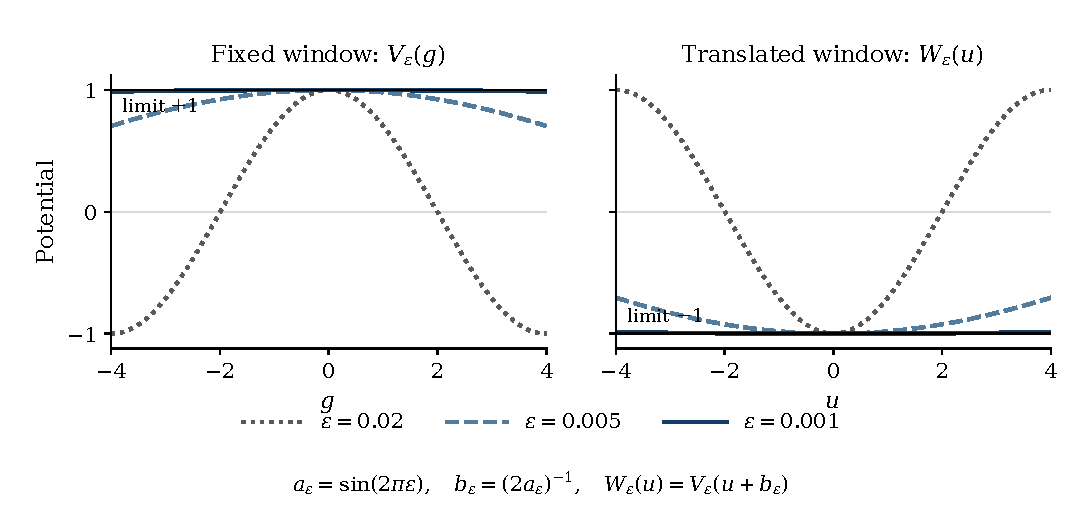
\includegraphics[width=\linewidth]{pictures/dynamical_potential_locality}
\caption{Fixed and translated windows for the shear-torus potentials,
with $V_\varepsilon=V_{z_\varepsilon}$ in the plot.
As $\varepsilon\downarrow0$, $V_{z_\varepsilon}$ tends to $1$ on each
fixed bounded window, while
$W_\varepsilon(u)=V_{z_\varepsilon}(u+b_\varepsilon)$ tends to $-1$,
with $b_\varepsilon\to\infty$. The curves show the explicit potentials,
not numerical approximations to their semigroups.}
\label{fig:dynamic_potential_windows}
\end{figure}

More explicitly, the conjugation identities are
\[
\begin{aligned}
U_{b_\varepsilon}(H_0+V_{z_\varepsilon})U_{b_\varepsilon}^{-1}
 &=H_0+W_\varepsilon,\\
U_{b_\varepsilon}S_{z_\varepsilon}(t)U_{b_\varepsilon}^{-1}
 &=e^{-t(H_0+W_\varepsilon)}.
\end{aligned}
\]
The potentials $W_\varepsilon$ are bounded by one. The same Duhamel
and dominated-convergence argument just proved, now comparing these
potentials directly with the constant $-1$, gives
\[
e^{-t(H_0+W_\varepsilon)}f\longrightarrow e^tP_tf
\qquad(f\in L^2).
\]
The member $S_{z_0}(t)=e^{-t}P_t$ is unchanged by translation.
Unitary invariance of the norm therefore implies, for any unit vector $f$,
\[
\liminf_{\varepsilon\downarrow0}
\|S_{z_\varepsilon}(t)-S_{z_0}(t)\|
\geq(e^t-e^{-t})\|P_tf\|_2.
\]
Here $\|P_t\|_{2\to2}=1$: the upper bound is known, and a unit vector
whose Fourier transform is supported in $\{|\xi|<\delta\}$ gives
$\|P_tf\|_2\geq e^{-t\delta^2}$. Letting $\delta\downarrow0$
proves the desired lower bound.

For the upper bound, the two-sided Gaussian estimates with $M=1$ give
\[
0\leq K_{z_\varepsilon}(t,x,y)-e^{-t}p_t(x-y)
\leq(e^t-e^{-t})p_t(x-y).
\]
Integration against $|f|$ and the $L^2$ contraction property of $P_t$
show that the operator norm of the difference is at most $e^t-e^{-t}$.
This proves \eqref{eq:dynamic_norm_discontinuity}. Nevertheless the
strong-continuity proposition applies, and the earlier weighted
Lipschitz estimate gives convergence of $k_t(z_\varepsilon,\cdot)$
to $k_t(z_0,\cdot)$ in every $C_a$. The loss of operator-norm
continuity comes from spatial translates moving out to infinity,
which are not controlled uniformly by convergence of this single row.

\subsection{Application to spectra over invariant subsystems}
The preceding counterexample concerns operator norm at individual phases.
There is a different useful consequence of the kernel estimates: spectral
continuity when entire invariant subsystems are compared. We give a direct
Euclidean heat-kernel proof of the localization argument in
\textcite[Lemmas~4.2--4.3 and Theorem~4.6]{BeckusTakase2025Spectral}.
Smooth cutoffs, the Gaussian first moment, and the localized operator
estimate supply the needed bounds. Only the self-adjoint spectral
calculus already used in the thesis is imported in this proof.

Let $\mathcal S$ be the collection of nonempty closed subsets of $Z$
invariant under every $T(g,\cdot)$. For $X,Y\in\mathcal S$, write
\[
d_H(X,Y)=\max\left\{
 \sup_{x\in X}\inf_{y\in Y}d_Z(x,y),
 \sup_{y\in Y}\inf_{x\in X}d_Z(x,y)\right\}.
\]
For each fixed $t>0$ define the compact spectral set
\[
\Sigma_t(X)=\overline{\bigcup_{z\in X}\sigma(e^{-tH_z})}
 \subseteq[0,e^{Mt}].
\]
The overline denotes closure in $\mathbb R$. Each spectrum is nonempty,
and operator positivity from spectral calculus and the norm bound for the heat
operator give the displayed inclusion, hence compactness.

\begin{lemma}[Averaged localization of a heat operator]
\label{lem:dynamic_spectral_localization}
Fix a real function $\chi\in C_c^1(B(0,1))$ with $\|\chi\|_2=1$,
and put $G_\chi=\|\nabla\chi\|_2$. For $R>0$ and $a\in\mathbb R^d$,
let $\chi_{a,R}(x)=R^{-d/2}\chi((x-a)/R)$, also denoting the
corresponding multiplication operator. Write $S_z=e^{-tH_z}$ for a
fixed $t>0$, and define
\[
B_t=e^{Mt}\sqrt{2dt}\,G_\chi.
\]
For every $f\in L^2$,
\[
\int\|\chi_{a,R}f\|_2^2\,da=\|f\|_2^2,\qquad
\left(\int\|[S_z,\chi_{a,R}]f\|_2^2\,da\right)^{1/2}
\leq \frac{B_t}{R}\|f\|_2.
\]
\end{lemma}
\Proof
Tonelli and the change of variable $u=(x-a)/R$ give the first identity.
Write $\chi_R=\chi_{0,R}$. The fundamental theorem of calculus
along a segment, followed by the triangle inequality in $L^2$, gives
\[
\|\chi_R(\cdot+r)-\chi_R\|_2
\leq |r|\|\nabla\chi_R\|_2
=\frac{|r|G_\chi}{R}.
\]
The commutator has the absolutely convergent kernel expression
\[
([S_z,\chi_{a,R}]f)(x)
=\int K_z(t,x,x+r)
 [\chi_R(x+r-a)-\chi_R(x-a)]f(x+r)\,dr.
\]
Absolute convergence at each $a,x$ follows from the Gaussian bound,
boundedness of $\chi_R$, and Cauchy--Schwarz against $f$.
All these integrands are jointly measurable. Put
$m_t=\int|r|p_t(r)\,dr\leq\sqrt{2dt}$. Scalar Cauchy--Schwarz,
with weight $|r|p_t(r)$, gives
\[
|([S_z,\chi_{a,R}]f)(x)|^2
\leq e^{2Mt}m_t\int\frac{p_t(r)}{|r|}
 |\chi_R(x+r-a)-\chi_R(x-a)|^2|f(x+r)|^2\,dr.
\]
The value at $r=0$ is irrelevant. This inequality is valid with an
infinite right side; the next calculation proves its integrability.
For each fixed $r$, integration in $a$ of the squared difference equals
$\|\chi_R(\cdot+r)-\chi_R\|_2^2$, independently of $x$.
Tonelli and translation invariance in $x$ therefore give
\[
\begin{split}
\int\|[S_z,\chi_{a,R}]f\|_2^2\,da
&\leq e^{2Mt}m_t\|f\|_2^2
  \int\frac{p_t(r)}{|r|}
  \|\chi_R(\cdot+r)-\chi_R\|_2^2\,dr\\
&\leq\frac{e^{2Mt}m_t^2G_\chi^2}{R^2}\|f\|_2^2
\leq\frac{B_t^2}{R^2}\|f\|_2^2.
\end{split}
\]
This proves the commutator estimate using only scalar
Cauchy--Schwarz and Tonelli.
\Done

\begin{corollary}[Spectral continuity of invariant subsystems]
\label{cor:dynamic_subsystem_spectra}
Under the original Lipschitz sampling and linear action-growth
hypotheses, fix the normalized cutoff from
Lemma~\ref{lem:dynamic_spectral_localization} and put
\[
Q_t=LCe^{Mt},\qquad b_d=c_d+\sqrt{d/2},\qquad
A_t=\max\{e^{Mt},\ B_t+Q_t(2t+b_dt^{3/2})\}.
\]
For all nonempty closed invariant subsets $X,Y$ of $Z$,
\[
\operatorname{dist}_H(\Sigma_t(X),\Sigma_t(Y))
\leq A_t d_H(X,Y)^{1/2}.
\]
\end{corollary}
\Proof
Let $\delta=d_H(X,Y)$. If $\delta=0$, compactness and closedness give
$X=Y$, and the claim is immediate. First suppose $0<\delta\leq1$.
Fix $z\in X$ and $\lambda\in\sigma(S_z)$. Since $S_z$ is bounded
self-adjoint, for every $\epsilon>0$ there is a unit vector $f$ with
$\|(S_z-\lambda)f\|_2<\epsilon$. To see this from the spectral theorem,
its spectral projection on $(\lambda-\epsilon,\lambda+\epsilon)$ is
nonzero; otherwise the spectral integral of $(s-\lambda)^{-1}$ would
supply a bounded inverse to $S_z-\lambda$. Normalize a nonzero vector
in that projection's range.

For any $R>0$, use
\[
(S_z-\lambda)\chi_{a,R}f
=\chi_{a,R}(S_z-\lambda)f+[S_z,\chi_{a,R}]f.
\]
The localization lemma and the triangle inequality in $L^2(da;L^2)$
give
\[
\left(\int\|(S_z-\lambda)\chi_{a,R}f\|_2^2\,da\right)^{1/2}
\leq\epsilon+B_t/R,
\qquad \int\|\chi_{a,R}f\|_2^2\,da=1.
\]
These are measurable functions of $a$; for example,
$a\mapsto\chi_{a,R}f$ is norm continuous, since translates of the
compactly supported continuous function $\chi_R$ vary continuously in
supremum norm. For every $\eta>0$, there is therefore an $a$ with
$\chi_{a,R}f\ne0$ and
\[
\frac{\|(S_z-\lambda)\chi_{a,R}f\|_2}{\|\chi_{a,R}f\|_2}
\leq\epsilon+B_t/R+\eta.
\]
Otherwise the squared numerator would be at least
$(\epsilon+B_t/R+\eta)^2$ times the squared denominator almost
everywhere, contradicting the two integral bounds.

Normalize this localized vector and translate it with
$(U_au)(x)=u(x+a)$. The resulting unit vector $v$ is supported in
$B(0,R)$. Translation of the potential gives
\[
U_aS_zU_a^{-1}=S_{T(a,z)}.
\]
Thus $z'=T(a,z)\in X$ and
$\|(S_{z'}-\lambda)v\|_2\leq\epsilon+B_t/R+\eta$.
Compactness of $Y$ supplies $w\in Y$ with $d_Z(z',w)\leq\delta$.
Proposition~\ref{prop:dynamic_local_operator_lipschitz}, applied to the
ball of radius $R$, yields
\[
\|(S_{z'}-S_w)v\|_2
\leq Q_t\,[t(1+R)+b_dt^{3/2}]\delta.
\]
Spectral calculus for the self-adjoint operator $S_w$ gives
$\operatorname{dist}(\lambda,\sigma(S_w))
\leq\|(S_w-\lambda)v\|_2$. Consequently
\[
\operatorname{dist}(\lambda,\Sigma_t(Y))
\leq\epsilon+\eta+B_t/R
 +Q_t[t(1+R)+b_dt^{3/2}]\delta.
\]
Let $\epsilon,\eta$ decrease to zero; the resulting bound is independent
of the chosen localizations and of $w$. Choose $R=\delta^{-1/2}$ and
use $\delta\leq\sqrt\delta$ to bound the right side by
\[
[B_t+Q_t(2t+b_dt^{3/2})]\sqrt\delta.
\]
The bound is uniform in $z\in X$ and $\lambda\in\sigma(S_z)$.
Distance to the closed set $\Sigma_t(Y)$ is continuous, so it extends
to every $\lambda\in\Sigma_t(X)$. Interchanging $X,Y$ gives the other
directed distance, proving the desired Hausdorff bound for
$0<\delta\leq1$.

Finally, if $\delta>1$, both nonempty spectral sets lie in $[0,e^{Mt}]$.
Their Hausdorff distance is at most $e^{Mt}\leq e^{Mt}\sqrt\delta$.
The stated maximum therefore works for every $\delta$.
\Done

\begin{corollary}[Qualitative spectral continuity under continuous sampling]
\label{cor:dynamic_subsystem_spectra_continuous}
Suppose only that $Z$ is a nonempty compact metric space, $T$ is a
continuous action of $\mathbb R^d$ on $Z$, and $v:Z\to\mathbb R$ is
continuous. For each fixed $t>0$, the map
$X\mapsto\Sigma_t(X)$ on nonempty closed invariant subsets of $Z$
is uniformly continuous for Hausdorff distance.
\end{corollary}
\Proof
Put $M=\|v\|_\infty$, and retain the cutoff and constant $B_t$ from
Lemma~\ref{lem:dynamic_spectral_localization}. That lemma uses only the
uniform Gaussian bound, so it remains valid under the present
hypotheses. For $R>0$, let $\chi_{B_R}$ be multiplication by the
indicator of $B(0,R)$, and define
\[
\omega_R(\delta)=\sup_{\substack{z,w\in Z\\d_Z(z,w)\leq\delta}}
 \|(S_z(t)-S_w(t))\chi_{B_R}\|_{2\to2},\qquad \delta\geq0.
\]
Proposition~\ref{prop:dynamic_strong_parameter_continuity} gives
operator-norm continuity of $z\mapsto S_z(t)\chi_{B_R}$.
Compactness of $Z$ makes this map uniformly continuous, and hence
$\omega_R(\delta)\to0$ as $\delta\downarrow0$ for each fixed $R$.

The localization and recentering argument in the proof of
Corollary~\ref{cor:dynamic_subsystem_spectra} uses the quantitative
hypotheses only when comparing the two operators on a vector supported
in $B(0,R)$. Replacing that comparison by the definition of
$\omega_R$ gives, for every $R>0$,
\[
\operatorname{dist}_H(\Sigma_t(X),\Sigma_t(Y))
 \leq \frac{B_t}{R}+\omega_R(d_H(X,Y)).
\]
Indeed, a localized approximate spectral vector for a phase in $X$
can be translated into $B(0,R)$; invariance keeps its translated phase
in $X$, and compactness of $Y$ supplies a phase within $d_H(X,Y)$.
The displayed modulus bounds the operator difference on that vector.
Letting the approximate-vector errors vanish, passing to spectral
closures, and interchanging $X,Y$ proves the inequality.
Given a positive error tolerance, first choose $R$ large and then
choose $d_H(X,Y)$ small. Both choices are independent of $X,Y$,
which proves uniform continuity.
\Done

\paragraph{Comparison with the general group theorem.}
The quantitative proof uses the original metric and linear action bound.
The following normalization additionally explains how the setting fits
\textcite[Theorem~1.3(a)]{BeckusTakase2025Spectral}, whose action bound
has coefficient one at the group identity.

\begin{lemma}[An adapted metric for the action]
\label{lem:dynamic_adapted_metric}
Under the original linear-growth hypothesis, put $C_0=\max\{1,C\}$ and
\[
d_*(z,w)=\sup_{g\in\mathbb R^d}
 \frac{d_Z(T(g,z),T(g,w))}{1+|g|}.
\]
Then $d_*$ is a metric with the same compact topology as $d_Z$, and
\[
d_Z\leq d_*\leq C_0d_Z,\qquad
 d_*(T(h,z),T(h,w))\leq(1+|h|)d_*(z,w).
\]
The sampling function $v$ remains Lipschitz with constant at most $L$.
\end{lemma}
\Proof
The assumed growth bound makes the supremum finite. Symmetry and the
triangle inequality follow from those of $d_Z$, taking suprema; the
term $g=0$ gives $d_*(z,w)\geq d_Z(z,w)$ and hence definiteness.
The two metric inequalities imply equivalence of their topologies and
preserve compactness. With $u=g+h$, the triangle inequality in
$\mathbb R^d$ gives
\[
1+|u|\leq(1+|u-h|)(1+|h|).
\]
Reindexing the supremum proves the action estimate. The sampling bound is
\[
|v(z)-v(w)|\leq Ld_Z(z,w)\leq Ld_*(z,w).
\]
\Done

Let $d_{H,*}$ denote Hausdorff distance induced by $d_*$.
The metric comparison gives $d_H\leq d_{H,*}\leq C_0d_H$ on
nonempty closed subsystems. With $\tau(g,z)=T(-g,z)$ and
$\kappa_t(r,z)=k_t(z,r)$, the operator convention in that theorem is
\[
(A_zf)(g)=\int\kappa_t(h-g,\tau(-g,z))f(h)\,dh
        =e^{-tH_z}f(g).
\]
The adapted action has bound $1+|g|$. Applying
Theorem~\ref{thm:dynamic_kernel_lipschitz} in $d_*$ gives an integrable
parameter-Lipschitz envelope, since it is a Gaussian times a linear
polynomial in $|r|$. The Gaussian bound also gives uniform integrability
and a uniform first moment, including suprema along translated orbits.
The heat operators are self-adjoint and hence normal. Finally,
$\mathbb R^d$ with its proper translation-invariant Euclidean metric
is unimodular and has ball volume $\omega_d r^d$, so the group's required
two-sided volume-growth condition holds. Thus the general theorem gives
another route to the result; its kernel hypotheses are verified rather
than assumed for the Schr\"odinger family.

\begin{corollary}[The bottom of the subsystem spectrum]
Under the baseline quantitative hypotheses, for $X\in\mathcal S$ let
\[
E(X)=\inf\bigcup_{z\in X}\sigma(H_z).
\]
Then $-M\leq E(X)\leq M$, and for every $t>0$,
\[
|E(X)-E(Y)|\leq\frac{e^{tM}}{t}A_t d_H(X,Y)^{1/2}.
\]
This statement concerns a spectral infimum; it does not assert that
there is an eigenvector at that energy.
\end{corollary}
\Proof
The operator inequality $H_z\geq-M$ proves the lower bound.
For any $\delta>0$, choose a unit vector whose Fourier transform is
supported in $\{|\xi|^2<\delta\}$. It belongs to $D(H_0)=D(H_z)$
and satisfies
\[
\langle H_zf,f\rangle
 =\int |\xi|^2|\widehat f(\xi)|^2\,d\xi
   +\int V_z(x)|f(x)|^2\,dx\leq\delta+M.
\]
Spectral calculus gives $\inf\sigma(H_z)\leq\langle H_zf,f\rangle$.
Letting $\delta\downarrow0$ proves the upper bound for each phase,
and hence for the nonempty subsystem.
Spectral mapping and the definition of infimum give
\[
\max\Sigma_t(X)=e^{-tE(X)}\in[e^{-tM},e^{tM}].
\]
Maxima of nonempty compact real sets differ by at most their Hausdorff
distance. On this interval the derivative of $-(1/t)\log s$ has
absolute value at most $e^{tM}/t$. Applying this Lipschitz bound to the
two maxima and then Corollary~\ref{cor:dynamic_subsystem_spectra}
proves the estimate.
\Done

The objects compared here are invariant subsystems, not arbitrary pairs
of individual phases. Moreover the spectral sets belong to the bounded
heat operators. By spectral mapping,
\[
\sigma(e^{-tH_z})=\overline{\{e^{-tE}:E\in\sigma(H_z)\}}.
\]
Passing back to unbounded energies uses a logarithm whose derivative
is unbounded near zero. No unweighted Hausdorff estimate for the
unbounded Schr\"odinger spectra, or for their intersections with a
sharp energy window, is asserted. The direct Euclidean argument specializes the cited localization
method; no new general spectral-continuity principle is claimed.

\begin{example}[The shear family and its limiting subsystem]
For the shear-torus family above, fix $t>0$ and define
\[
X_\varepsilon=\{[\varepsilon,y]:y\in\mathbb R/\mathbb Z\},\qquad
X_0=\{[0,y]:y\in\mathbb R/\mathbb Z\}.
\]
For $0<\varepsilon<1/4$, the nonzero speed
$a_\varepsilon=\sin(2\pi\varepsilon)$ makes the orbit of
$z_\varepsilon$ equal to $X_\varepsilon$: as $g$ ranges over
$\mathbb R$, $ga_\varepsilon$ ranges over $\mathbb R$.
The quotient Euclidean metric gives
$d_H(X_\varepsilon,X_0)=\varepsilon$, by matching second coordinates
and minimizing the first-coordinate distance. But the orbit of $z_0$
is only the singleton $\{z_0\}$, not $X_0$.

All phases in $X_\varepsilon$ give unitarily equivalent operators:
translation by $b$ conjugates $H_z$ to $H_{T(b,z)}$, and the action
is transitive on this circle. Thus
$\Sigma_t(X_\varepsilon)=\sigma(S_{z_\varepsilon}(t))$.
On $X_0$ each potential is the constant $\cos(2\pi y)$.
The Fourier multiplier $|\xi|^2$ has essential range $[0,\infty)$,
so $\sigma(H_0)=[0,\infty)$. Spectral mapping therefore gives
\[
\sigma(e^{-t(H_0+c)})=[0,e^{-tc}]\quad(c\in\mathbb R),
\qquad \Sigma_t(X_0)=[0,e^t].
\]
Corollary~\ref{cor:dynamic_subsystem_spectra} now proves
\[
\operatorname{dist}_H\bigl(\sigma(S_{z_\varepsilon}(t)),[0,e^t]\bigr)
 \leq A_t\sqrt{\varepsilon}.
\]
In contrast, $\sigma(S_{z_0}(t))=[0,e^{-t}]$. The triangle inequality
for Hausdorff distance, applied with this fixed interval, yields
\[
\lim_{\varepsilon\downarrow0}
\operatorname{dist}_H\bigl(\sigma(S_{z_\varepsilon}(t)),
                         \sigma(S_{z_0}(t))\bigr)=e^t-e^{-t}.
\]
Thus even the phase spectra are discontinuous here. The subsystem
spectra converge to the spectrum of the limiting circle, which is
larger than the orbit of the limiting phase. This conclusion follows from the spectral localization argument;
the earlier operator-norm limit has its separate direct proof.
\end{example}

\ifdefined\qwertyflag
\undef\qwertyflag
\end{document}
\fi



\chapter*{Conclusion}
\addcontentsline{toc}{chapter}{Conclusion}
For bounded real potentials the heat semigroup has a specified jointly
continuous, positive kernel with two-sided Gaussian bounds. Under the
stated dynamical hypotheses, its canonical kernel is Lipschitz in the
parameter, with an explicit Gaussian-weighted estimate. In particular,
every fixed exponential spatial weight is allowed at positive times.
The argument extends to Hölder sampling functions, and isometric
actions admit a sharper bound. The two translation conventions give
equivalent formulations when the definition of the potential is changed
consistently.

The arguments separate three issues that require different hypotheses:
uniqueness of a PDE solution in a growth class, uniqueness of a continuous
kernel representative under full measure support, and uniform parameter
regularity after integration against Gaussian kernels. Neither separate
continuity nor an almost-everywhere operator identity alone substitutes
for the pointwise assertions proved here. The canonical kernel cannot be continuous at time zero in these weighted
supremum norms. The operator family is strongly continuous in its
parameter, uniformly on bounded time intervals; the shear-torus example
proves that operator-norm continuity can nevertheless fail even under
the original Lipschitz hypotheses. Thus the distinction between a
canonical row and the full covariant operator has a concrete consequence.

\printbibliography[heading=bibintoc,title={References}]
\end{document}

